\chapter{Results and Analysis}

The invariant mass distribution of the real data is shown in Figure \ref{inv_mass_data}. For simplicity, it was assumed that the invariant mass distribution shown in the figure is composed only of the decays originating from the signal and control channels and from the combinatorial background. The peak in Figure \ref{inv_mass_data} is caused by $B^{0} \rightarrow \psi(2S)K_{s}^{0}$ decays, while the signal decay ($B_{s}^{0} \rightarrow \psi(2S)K_{s}^{0}$) cannot be observed as it is submerged by combinatorial background.\\   
    \begin{figure}[H]
        \centering
        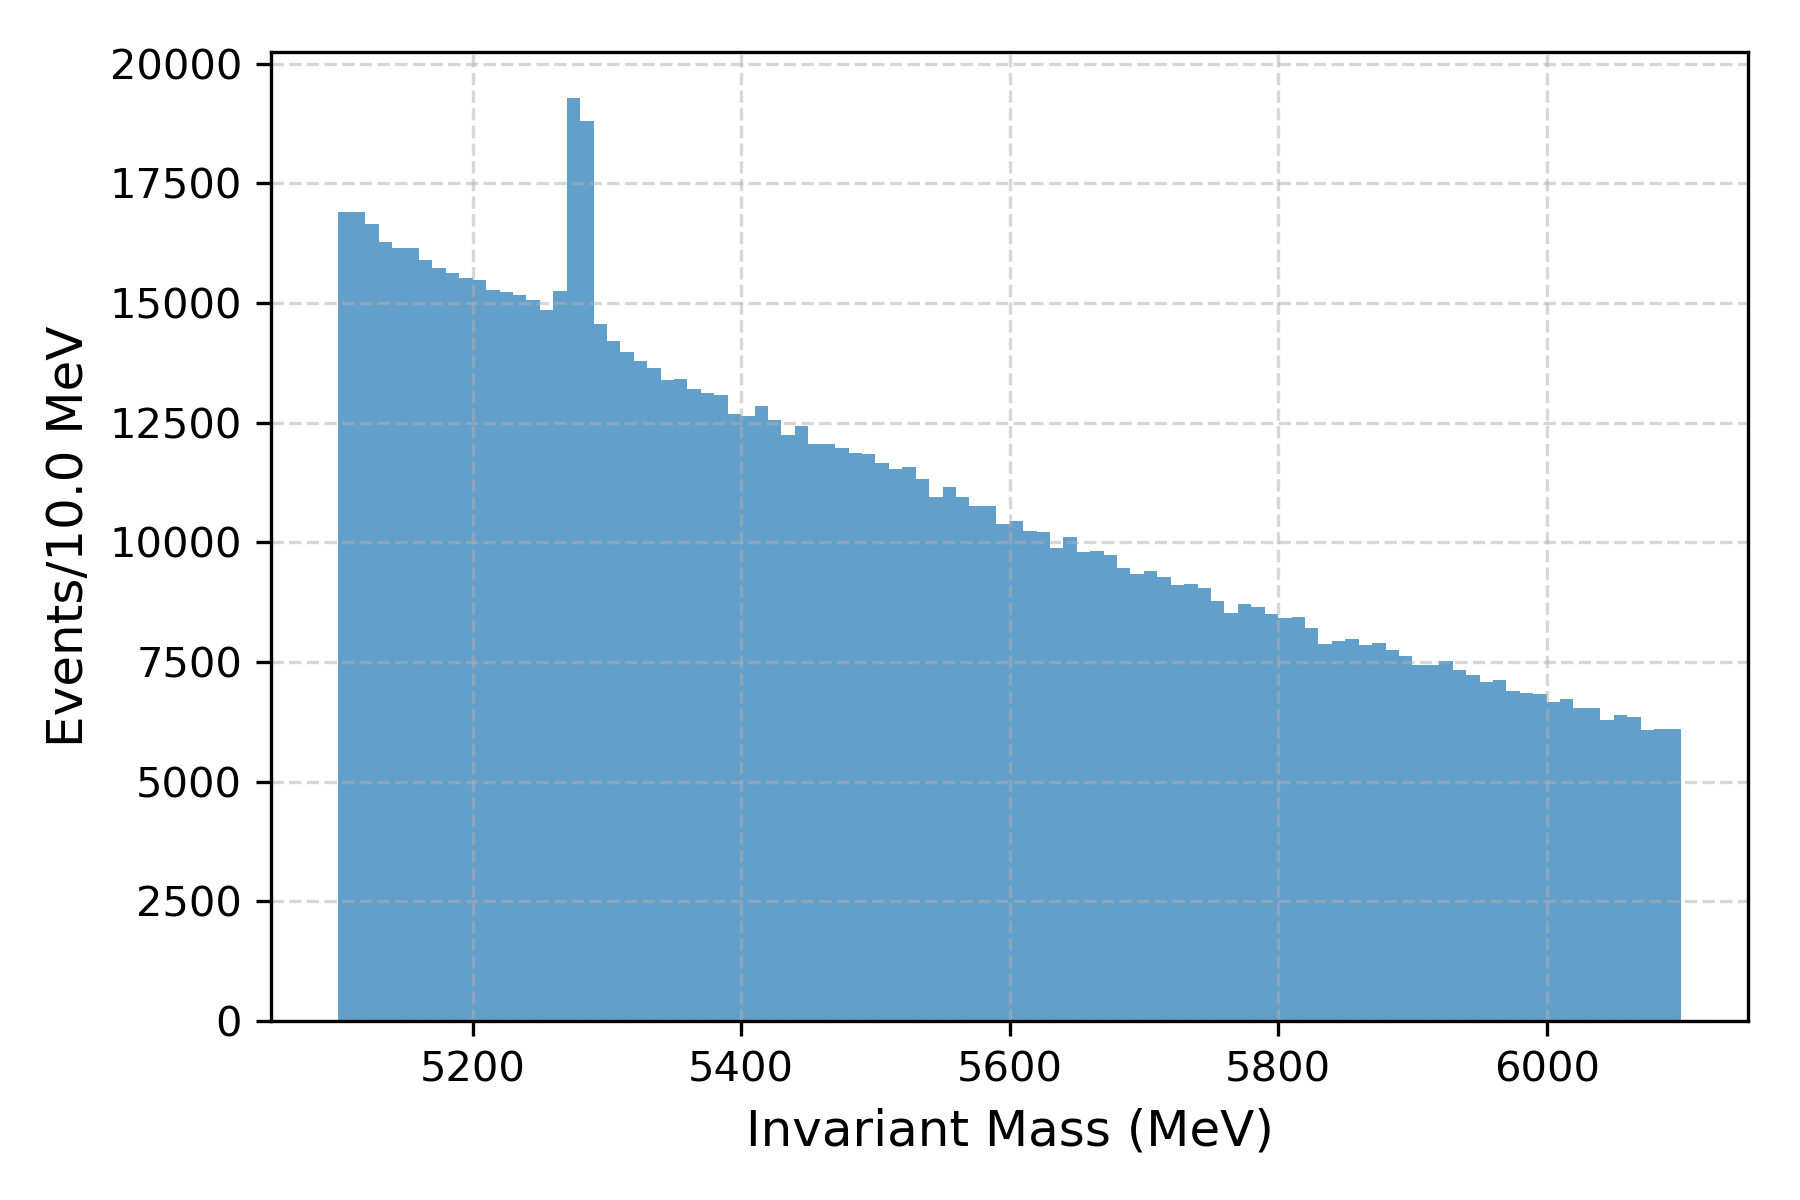
\includegraphics[width=0.7\linewidth]{Figure/2_data_invariant_mass_distribution.png}
        \caption{Reconstructed invariant mass distribution of the real data set.}
        \label{inv_mass_data}
    \end{figure}

    \section{Signal Region and Background Sample}
    In order to define the signal region in the real dataset, a selection was made in the real dataset was made with the help of the signal simulation dataset. First, a window containing $99\%$ of the data was found in the signal dataset as shown Figure \ref{in_mass_sig}.\\

    \begin{figure}[H]
        \centering
        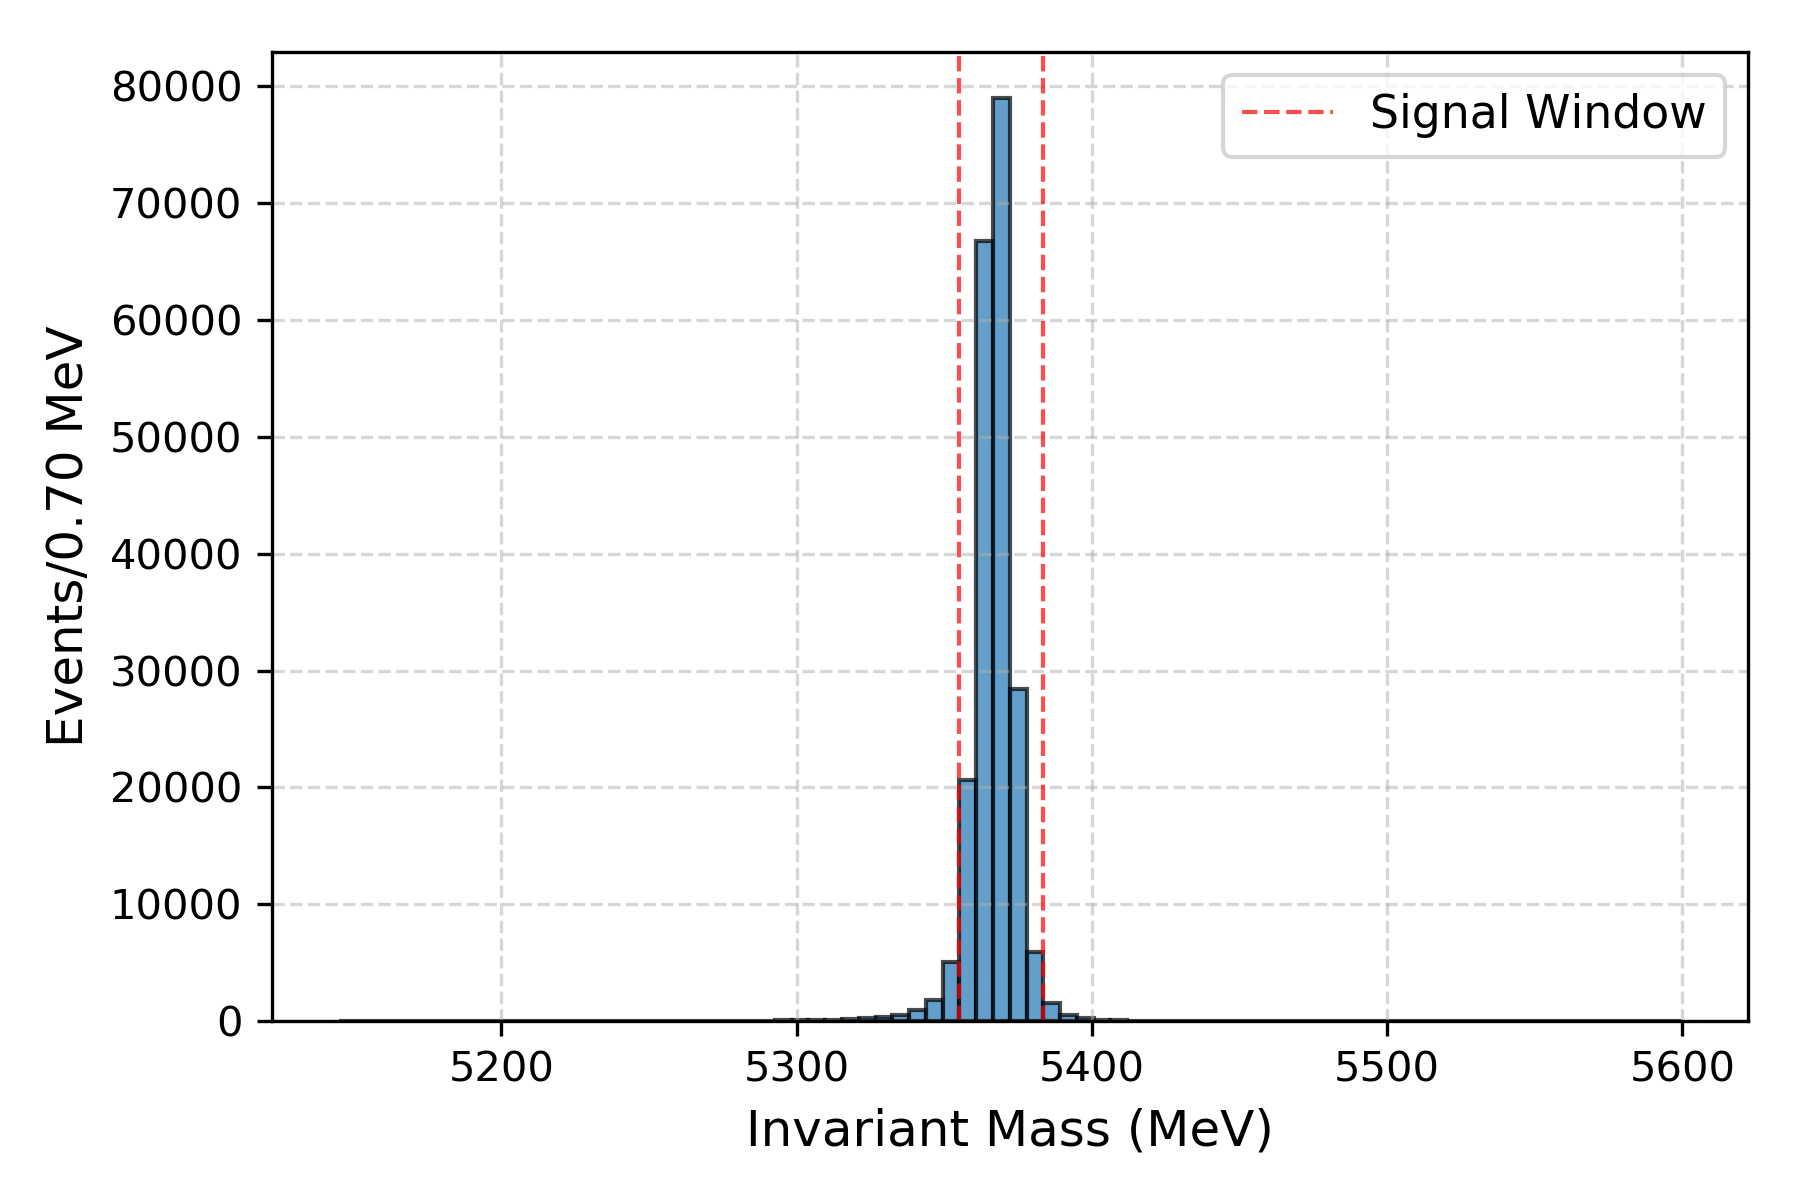
\includegraphics[width=0.7\linewidth]{Figure/3_signal_invariant_mass_distribution_99_data.png}
        \caption{Reconstructed invariant mass distribution of the signal simulation.}
        \label{in_mass_sig}
    \end{figure}
    Afterwards, this window is implemented in the invariant mass distribution of the real dataset as shown in Figure \ref{inv_mass_data_99}\\
    \begin{figure}[H]
        \centering
        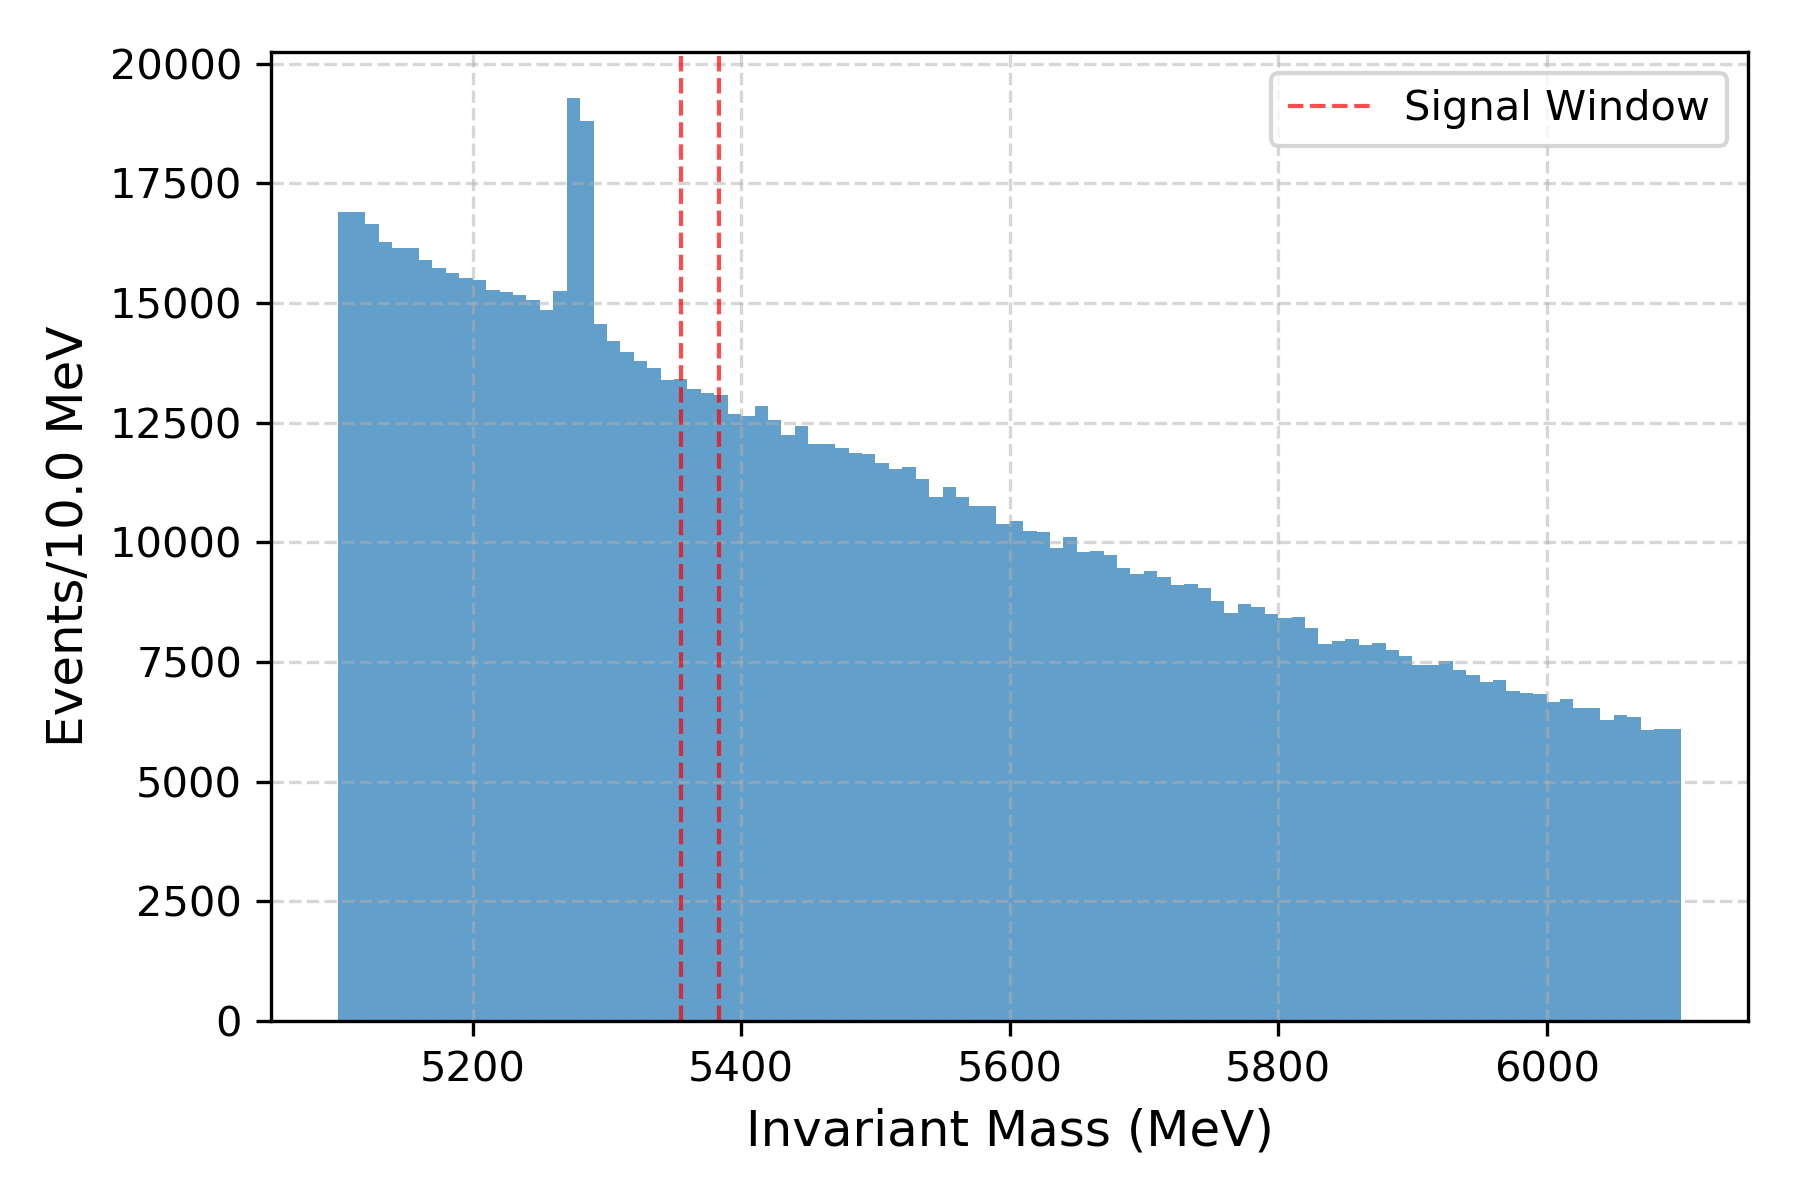
\includegraphics[width=0.7\linewidth]{Figure/4_data_invariant_mass_distribution.png}
        \caption{Implemented signal region in the real data set invariant mass distribution.}
        \label{inv_mass_data_99}
    \end{figure}
    
    The two Monte Carlo simulations do not contain any background, so the background must be identified within the real data set. So, to train the MVA to recognize background, background from the real data sample shall be used. Hence, the upper side band (USB) of the real data set was taken as the background sample, i.e. all the data in the real data set that have invariant mass higher than the right side of the signal region. The signal simulation dataset and the background candidates obtained from the USB are used for the MVA training.\\

    In the real data set, there is a column with weights, which if used gives the pure $B^{0}$ events. The figure below shows the distribution with and without these weights.\\ 
    
    \begin{figure}[H]
        \centering
        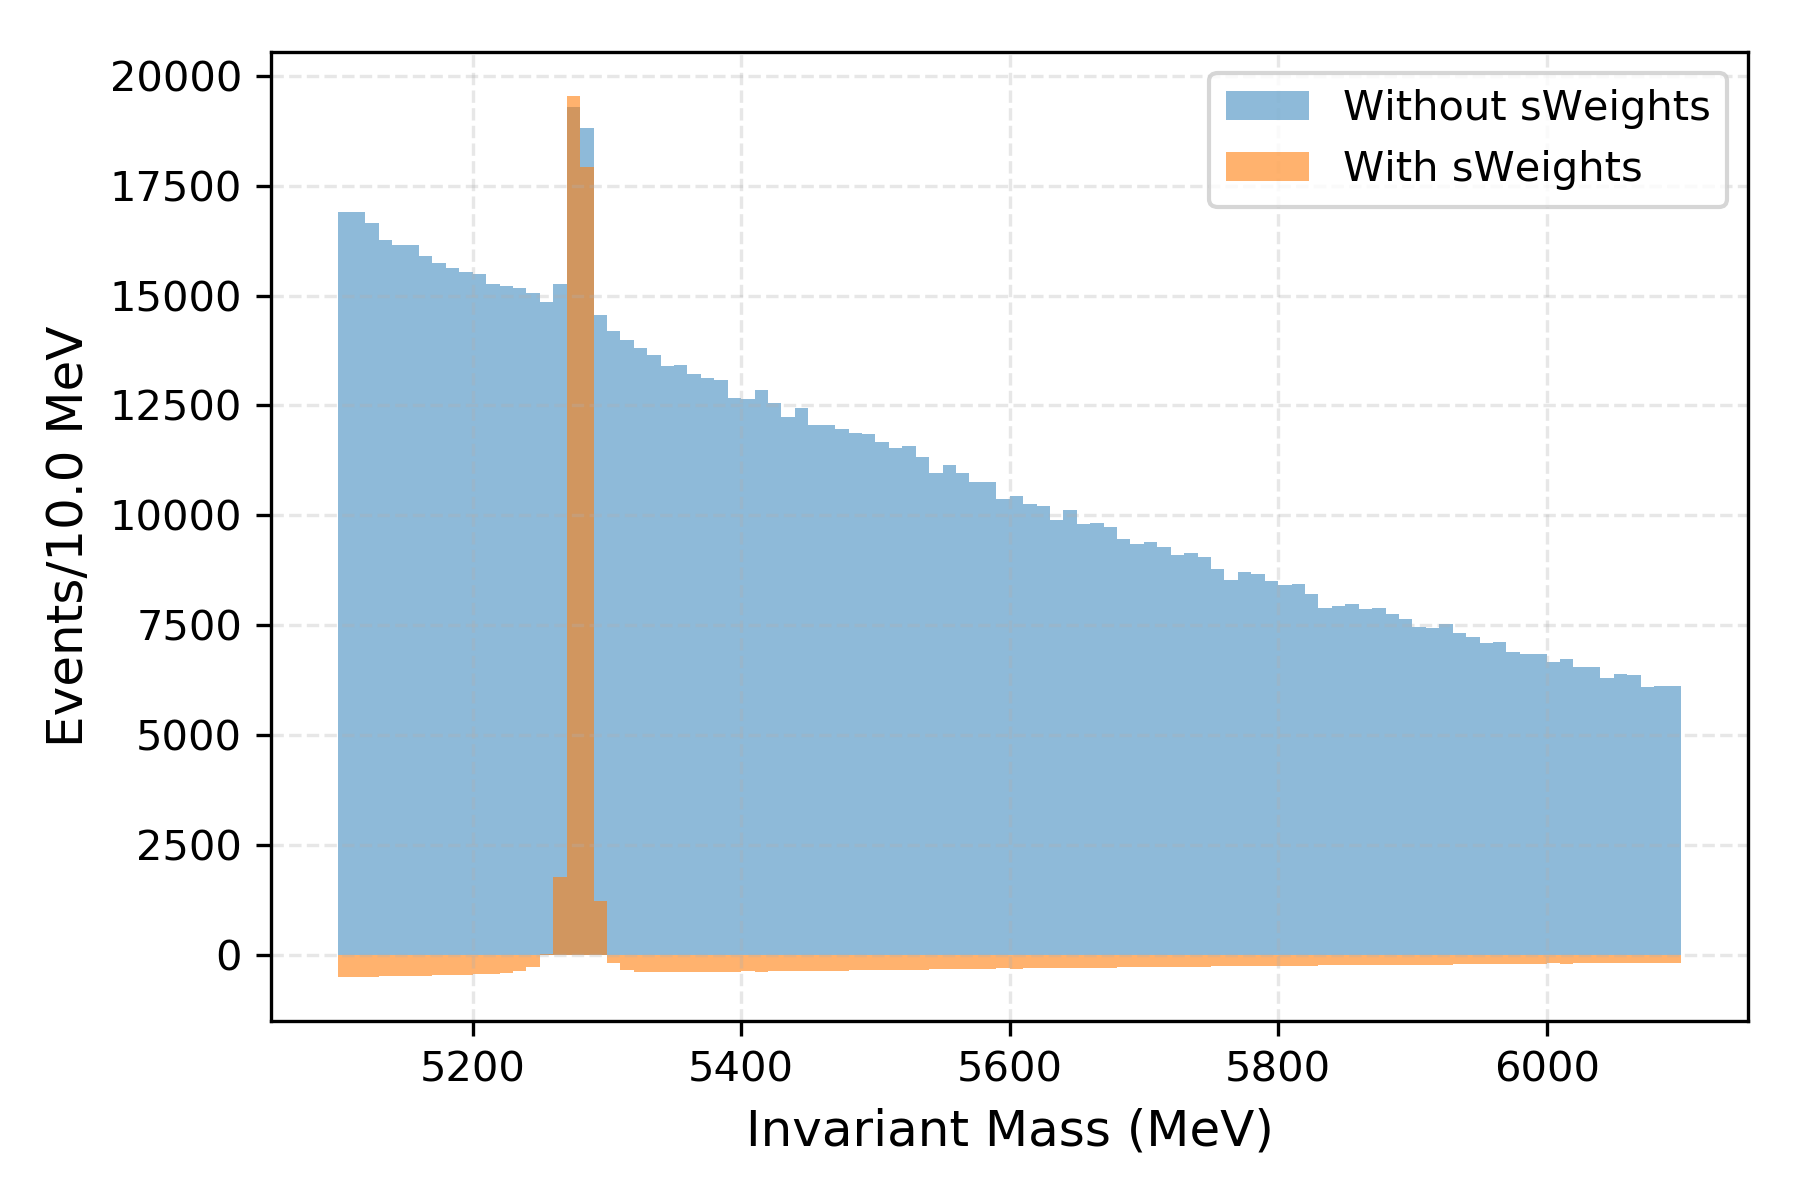
\includegraphics[width=0.7\linewidth]
        {Figure/5_data_invariant_mass_distribution_sWeights.png}
        \caption{Invariant mass distribution as returned by the trigger line (blue) and invariant mass distribution of the $B^{0}$ candidates, highlighted using background subtraction (s-weights) whights (orange).}
        \label{pure}
    \end{figure}

%$B_{s}^{0} \rightarrow \psi(2S)K_{s}^{0}$
    
    \section{Feature Selection}
    Even after using the weights there are many differences in the distribution due to various reasons. A large number of features will make the model slow and also lead to overfitting whereas a small amount of features will make poor predictions. Not all of the features in the dataset contain useful information. In order to select suitable features, the KS test was used.\\
    
    Hence, features which satisfies the following conditions must be used for training the model:
    \begin{enumerate}
        \item Reasonable agreement between data and simulation (otherwise the classifier only learns to distinguish data from simulation instead of signal from background).
        \item Strong discrimination between signal (simulation) and background (USB).
        \item Uncorrelated to the invariant mass of the $B_{s}^{0}/B^{0}$
      candidate.
    \end{enumerate}
    Using the KS test, 27 suitable features were found based on the above criteria. In order to find similarity between the $B^{0}$ simulation and $B^{0}$ data, a threshold KS < 0.05 had been used and to distinguish between the signal and the background a threshold of KS > 0.2 had been used. In this test, the KS metric had values [0, 1] where 0 means that the distributions are identical and 1 means that the distributions are completely different. The thresholds used in the analysis are achieved via exploratory analysis.

    \section{Training the Classifier and Optimization}
    The machine learning model used in the analysis was XGBClassifier, which is a supervised learning model. Since, the number of background data is very large compared to the number of signal data, weights has been used to make accurate predictions. Because, imbalanced data can lead to misleading or biased classifications. Afterwards, hyperparameter optimization was done to slightly improve the performance of the model. In this case, RandomizedSearchCV, which is a hyperparameter tuning technique provided by scikit-learn library, had been used. The best parameters obtained from the optimizations are shown in Table \ref{hyperparameter}.\\
    
\begin{table}[H]
        \centering
        \begin{tabular}{cc}
            \hline
            Parameters & Best Values\\
            \hline
             \texttt{n\_estimators} & $1000$ \\
             \texttt{max\_depth} & $6$ \\
             \texttt{learning\_rate} &  $0.1$ \\
             \texttt{lambda} & $1$ \\
             \hline
        \end{tabular}
        \caption{Best parameters obtained from hyperparameter optimization.}
        \label{hyperparameter}
    \end{table}
    
    The evaluation of the model can be done with the following receiver operating characteristic (ROC) curve and confusion matrix.\\

    \begin{figure}[H]
        \centering
        \begin{subfigure}[b]{0.49\linewidth}
            \centering
            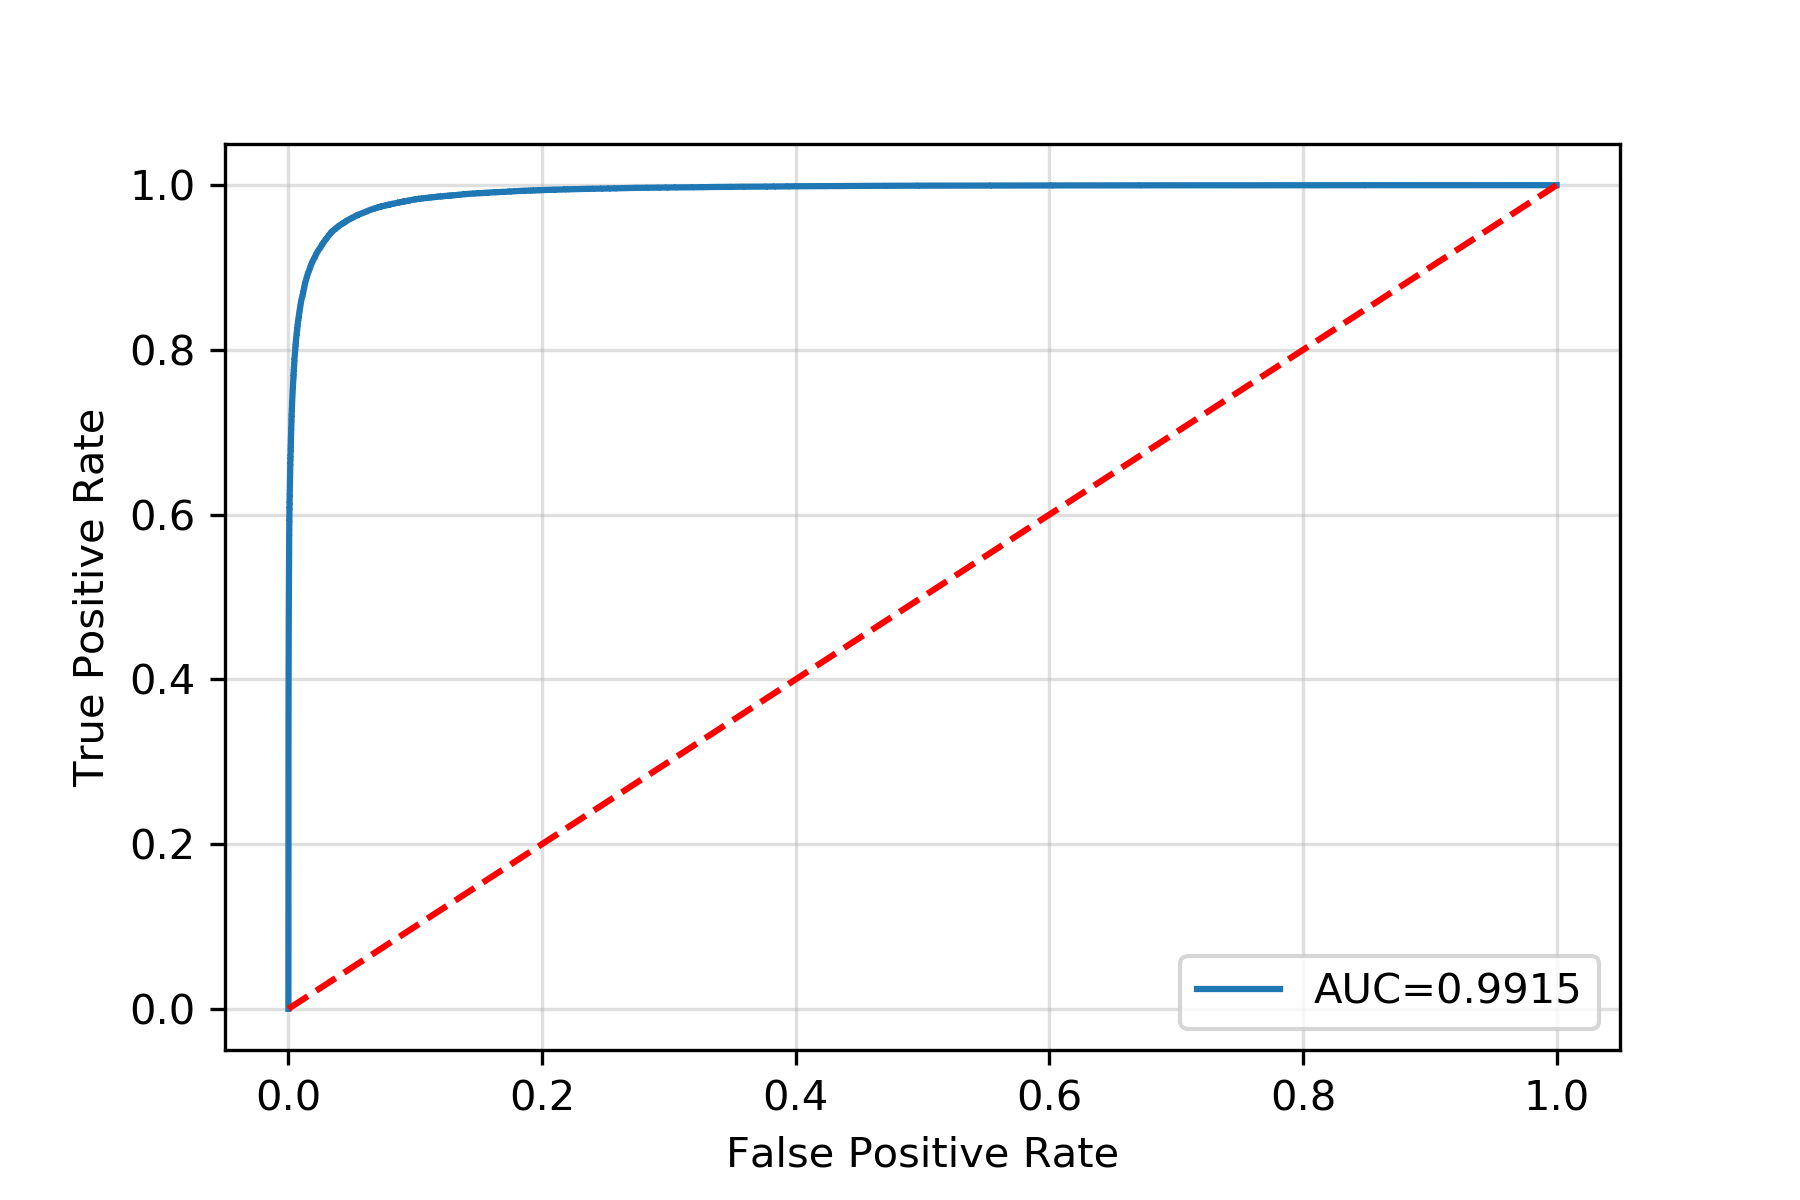
\includegraphics[width=0.95\linewidth]{Figure/roc_curve.png}
            \caption{ROC curve with the total area under the curve (AUC) value.}
            \label{roc_curve}
        \end{subfigure}
        \hfill
        \begin{subfigure}[b]{0.49\linewidth}
            \centering
            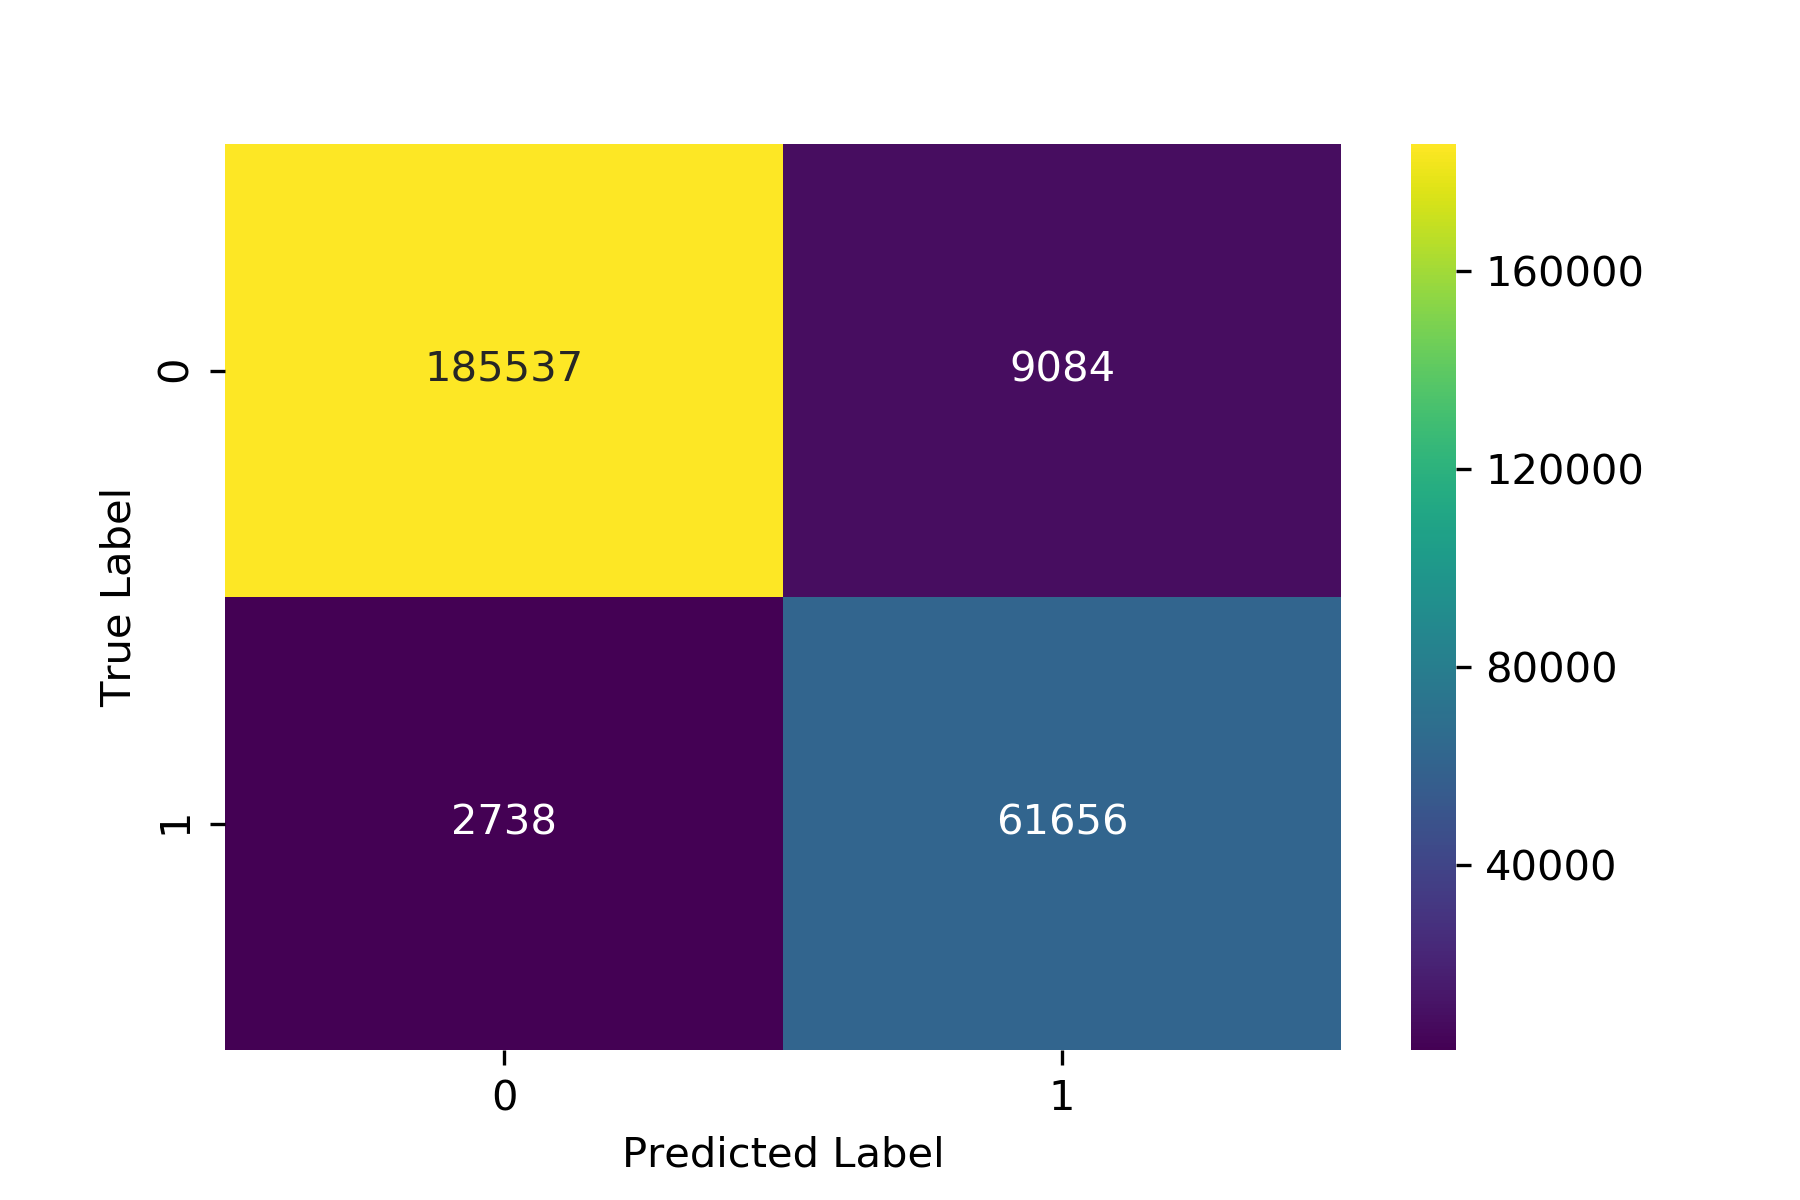
\includegraphics[width=0.95\linewidth]{Figure/confusion_matrix.png}
            \caption{Confusion matrix.}
            \label{confusion_matrix}
        \end{subfigure}
        \caption{Evaluation of the BDT model.}
    \end{figure}
    Both the confusion matrix and AUC score suggest that the model was trained well. The AUC score is especially useful in this scenario, when the dataset is heavily dominated by background samples. Another parameter is the boosted decision tree (BDT) score, which is a numeric output of a boosted decision tree classifier such as XGBClassifier, that reflects how strongly the model classifies a given event as signal or background. The distribution of the BDT score is shown in Figure \ref{dist}.\\
    
    \begin{figure}[H]
        \centering
        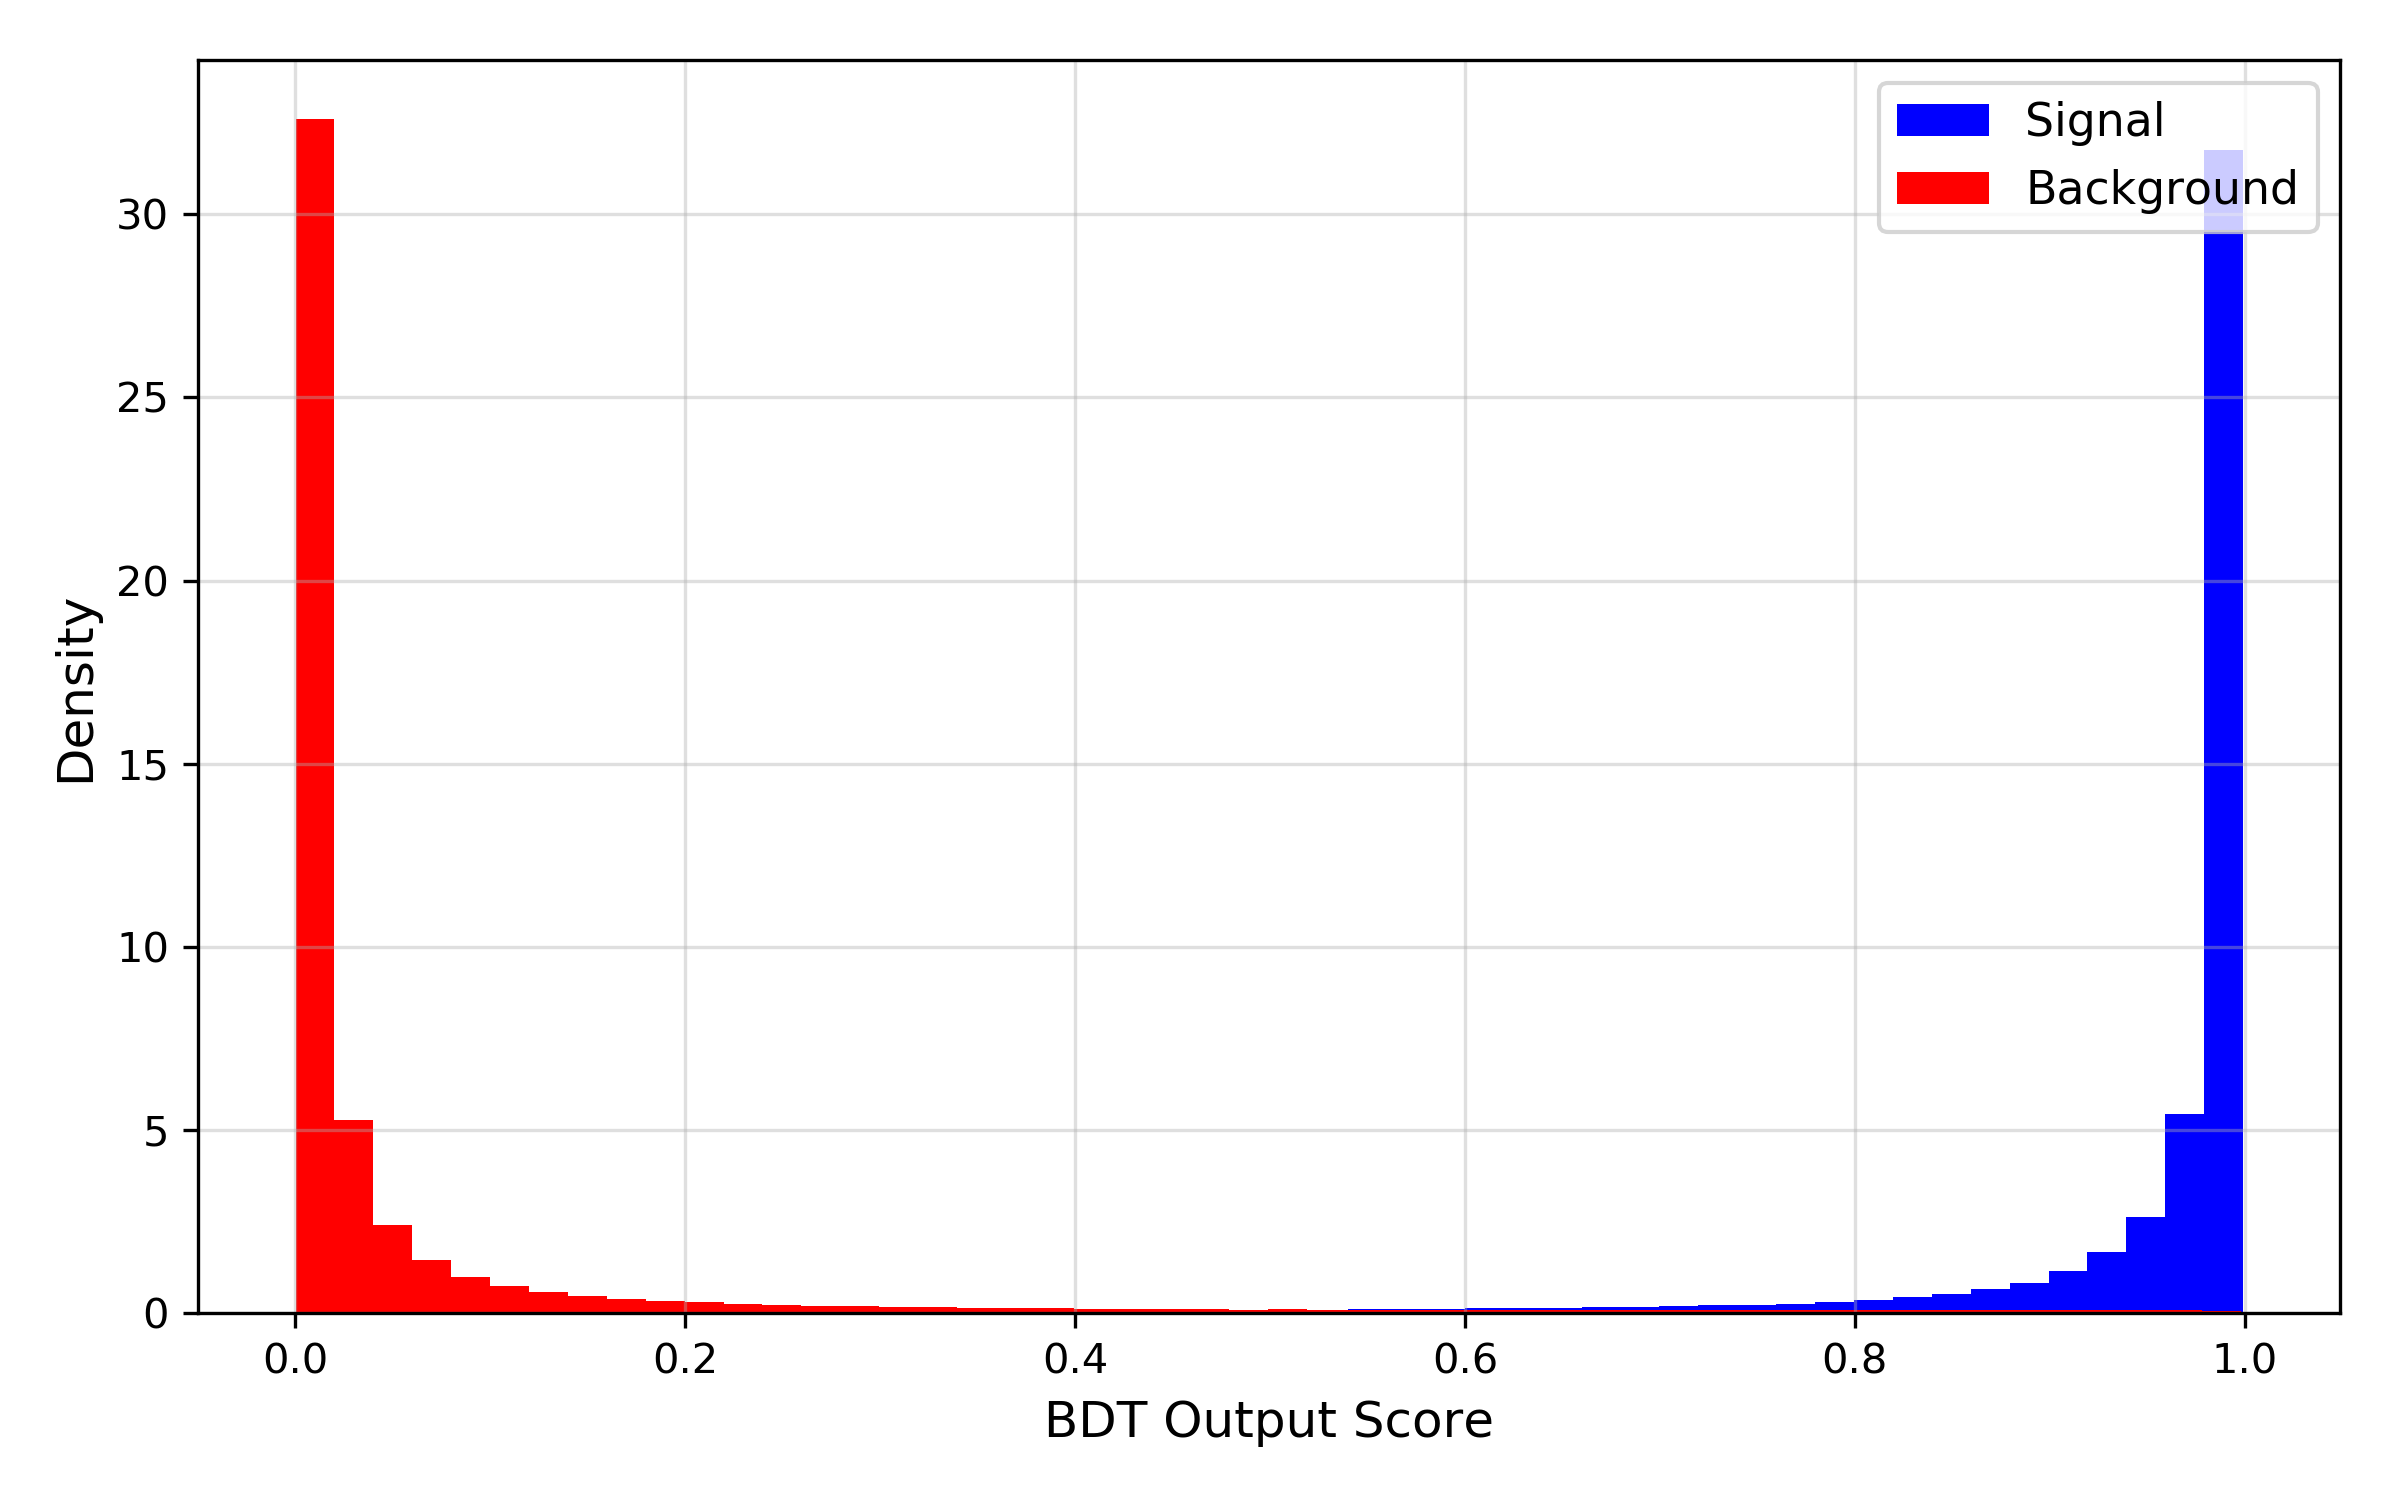
\includegraphics[width=0.7\linewidth]{Figure/6_BDT_Score.png}
        \caption{Distribution of the BDT output for background and signal samples.}
        \label{dist}
    \end{figure}

    From Figure \ref{sig_vs_thres}, it can be easily found that the best cut value which maximizes the Punzi FOM is $0.9919$. A plot of significances vs. threshold is shown in Figure \ref{sig_vs_thres}.

    \begin{figure}[H]
        \centering
        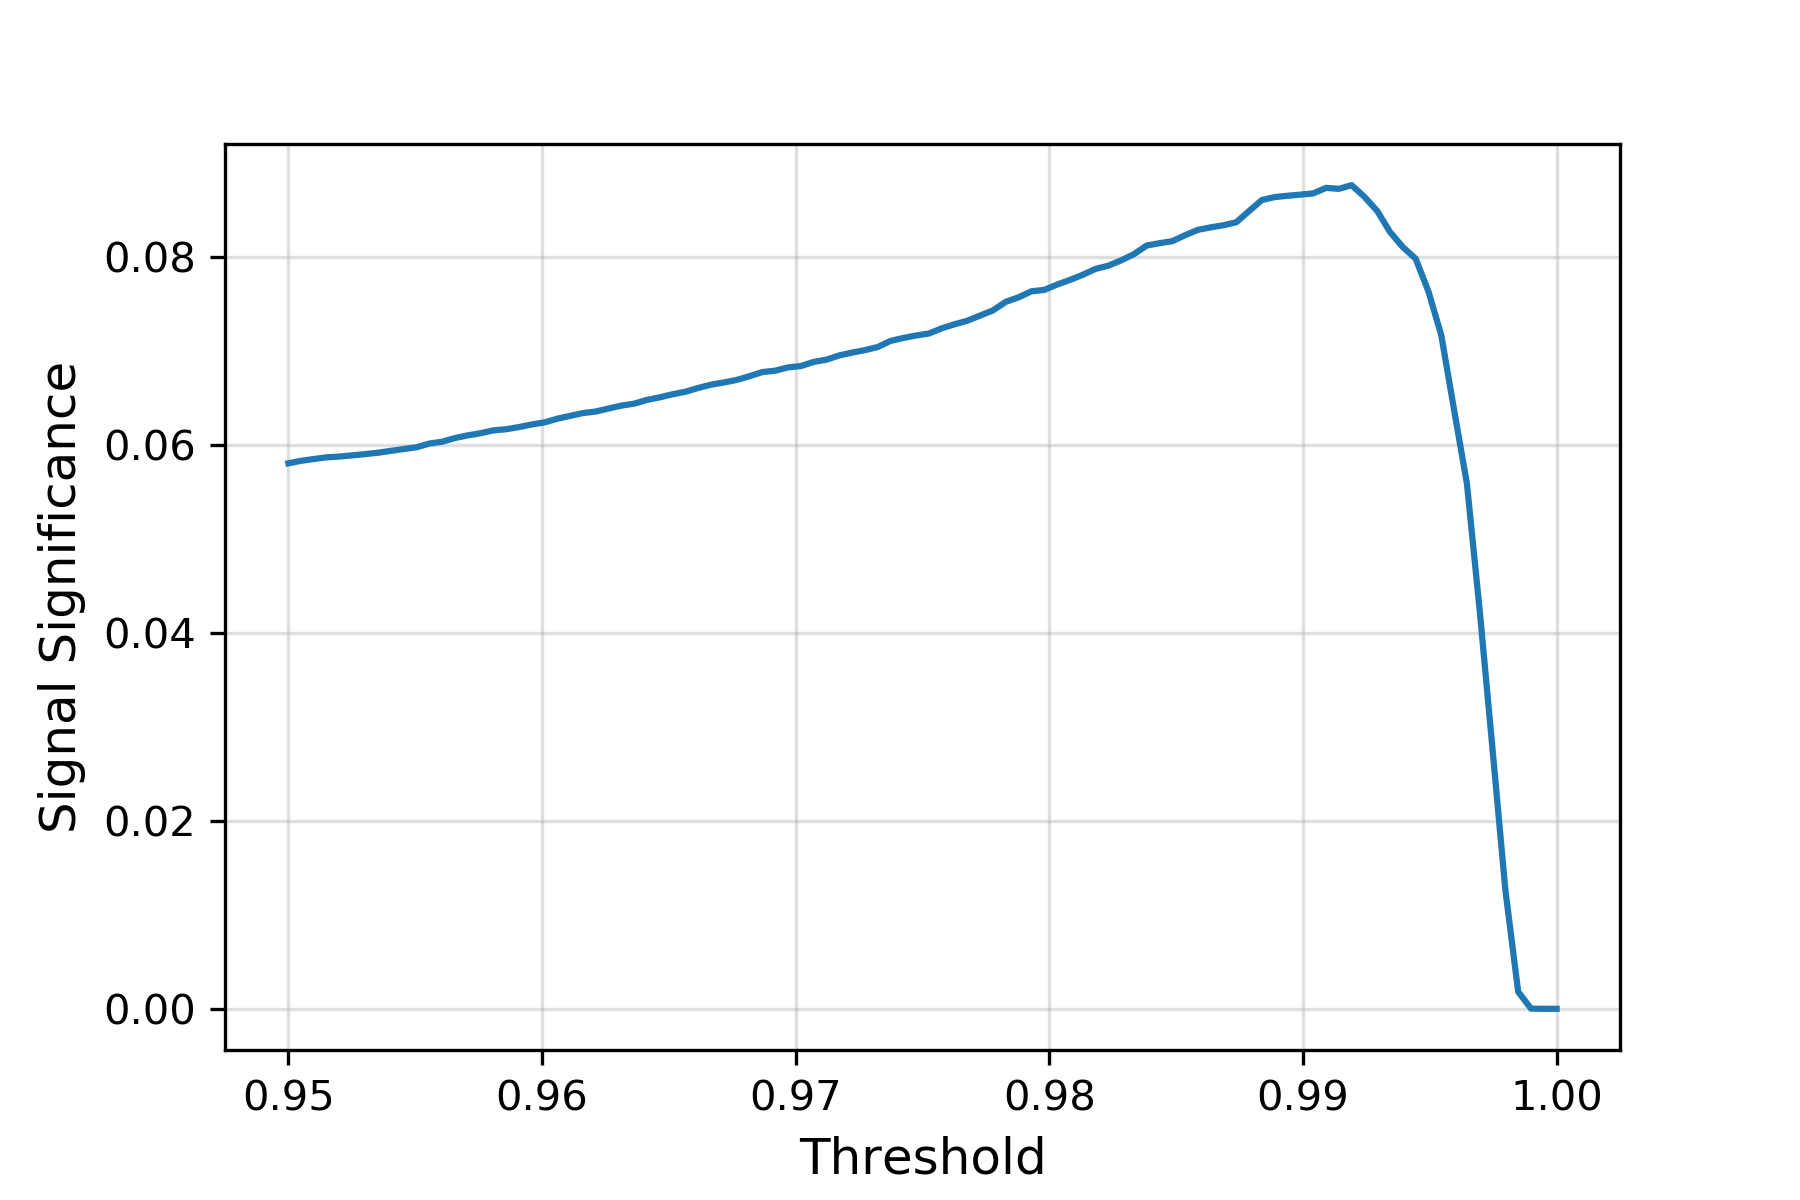
\includegraphics[width=0.5\linewidth]{Figure/7_significance_vs_threshold.png}
        \caption{Plot of Punzi FOM as a function of threshold.}
        \label{sig_vs_thres}
    \end{figure}
    Applying this best cut, a purer plot of the real data sample can be obtained as shown in Figure \ref{last_inv}.\\
    \begin{figure}[H]
        \centering
        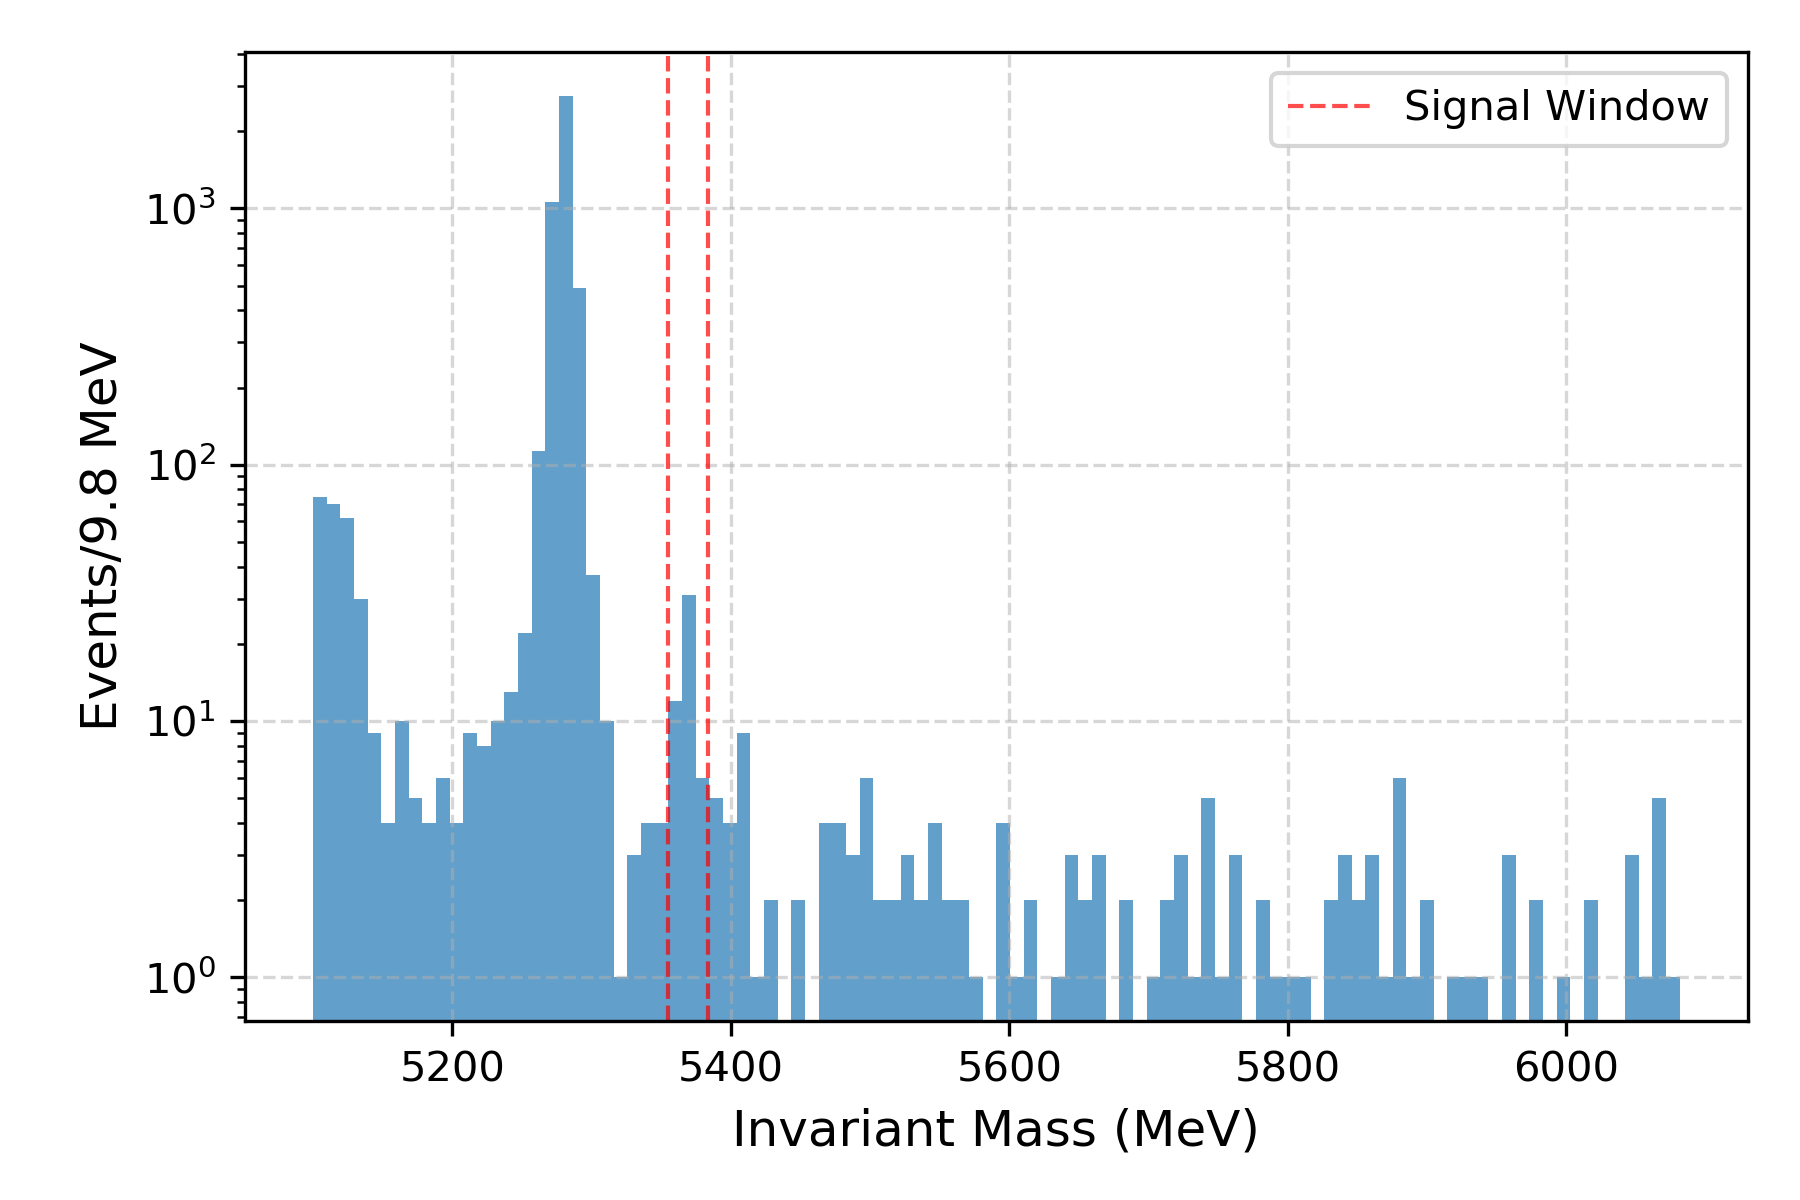
\includegraphics[width=0.5\linewidth]{Figure/8_data_invariant_mass_distribution.png}
        \caption{Selected mass distribution of the real data set.}
        \label{last_inv}
    \end{figure}
    In Figure \ref{last_inv}, two peaky structures can be observed in the regions where we expect the  $B_{s}$ and $B^{0}$ mass peaks.

    \section{Finding the Signal in the Data Sample}
    If peaks are fitted in the signal and control simulation using Gaussian function, then Figure \ref{fit_signal_peak} and \ref{fit_control_peak} are obtained. A Gaussian function has been used to fit peaks in signal and control simulations because it models the symmetric distribution of reconstructed quantities around their true values due to detector resolution, which provides with simple and symmetric signal shape. The formula for a Gaussian function (also known as the normal distribution) is:\\

    \begin{align}
        f(x) = A \cdot e^{-\frac{(x - \mu)^2}{2\sigma^2}}
    \end{align}
    where A is the height of the peak (amplitude), $\mu$ is the mean, $\sigma$ is the standard deviation and $e$ is the Euler's number.\\
    \begin{figure}[H]
        \centering
        \begin{subfigure}[b]{0.49\linewidth}
            \centering
            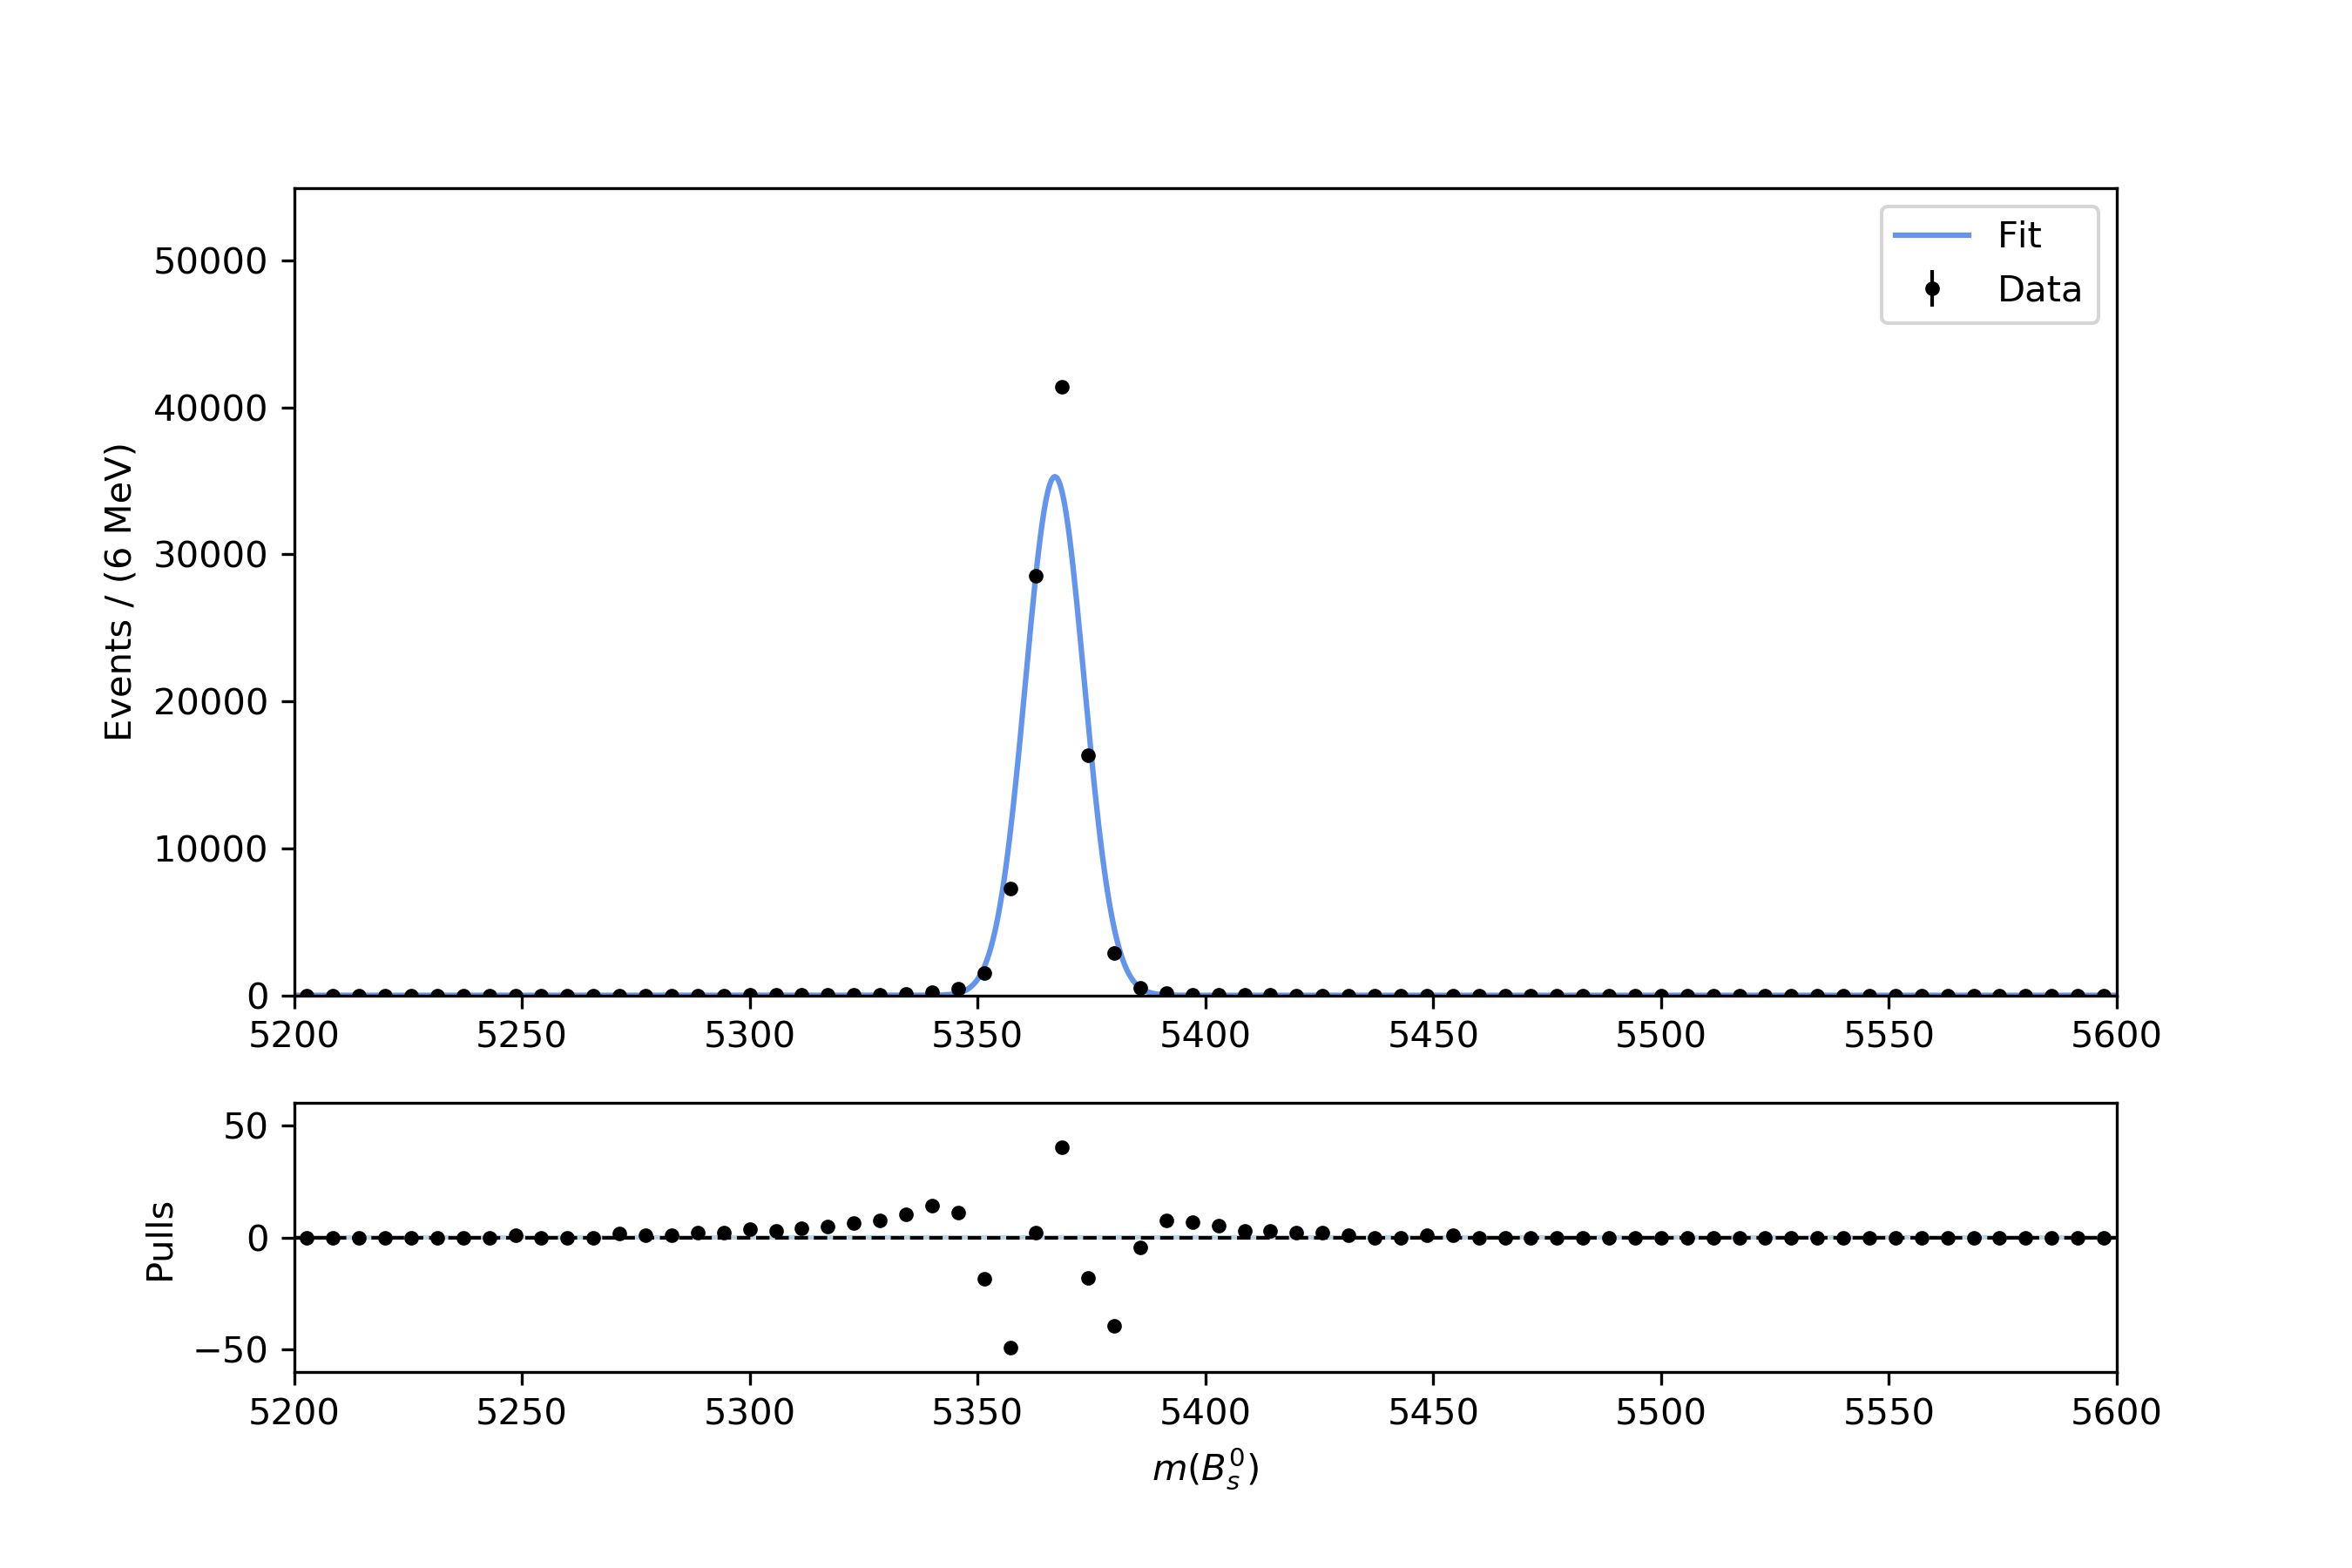
\includegraphics[width=0.99\linewidth]{Figure/second.png}
            \caption{Signal simulation.}
            \label{fit_signal_peak}
        \end{subfigure}
        \hfill
        \begin{subfigure}[b]{0.49\linewidth}
            \centering
            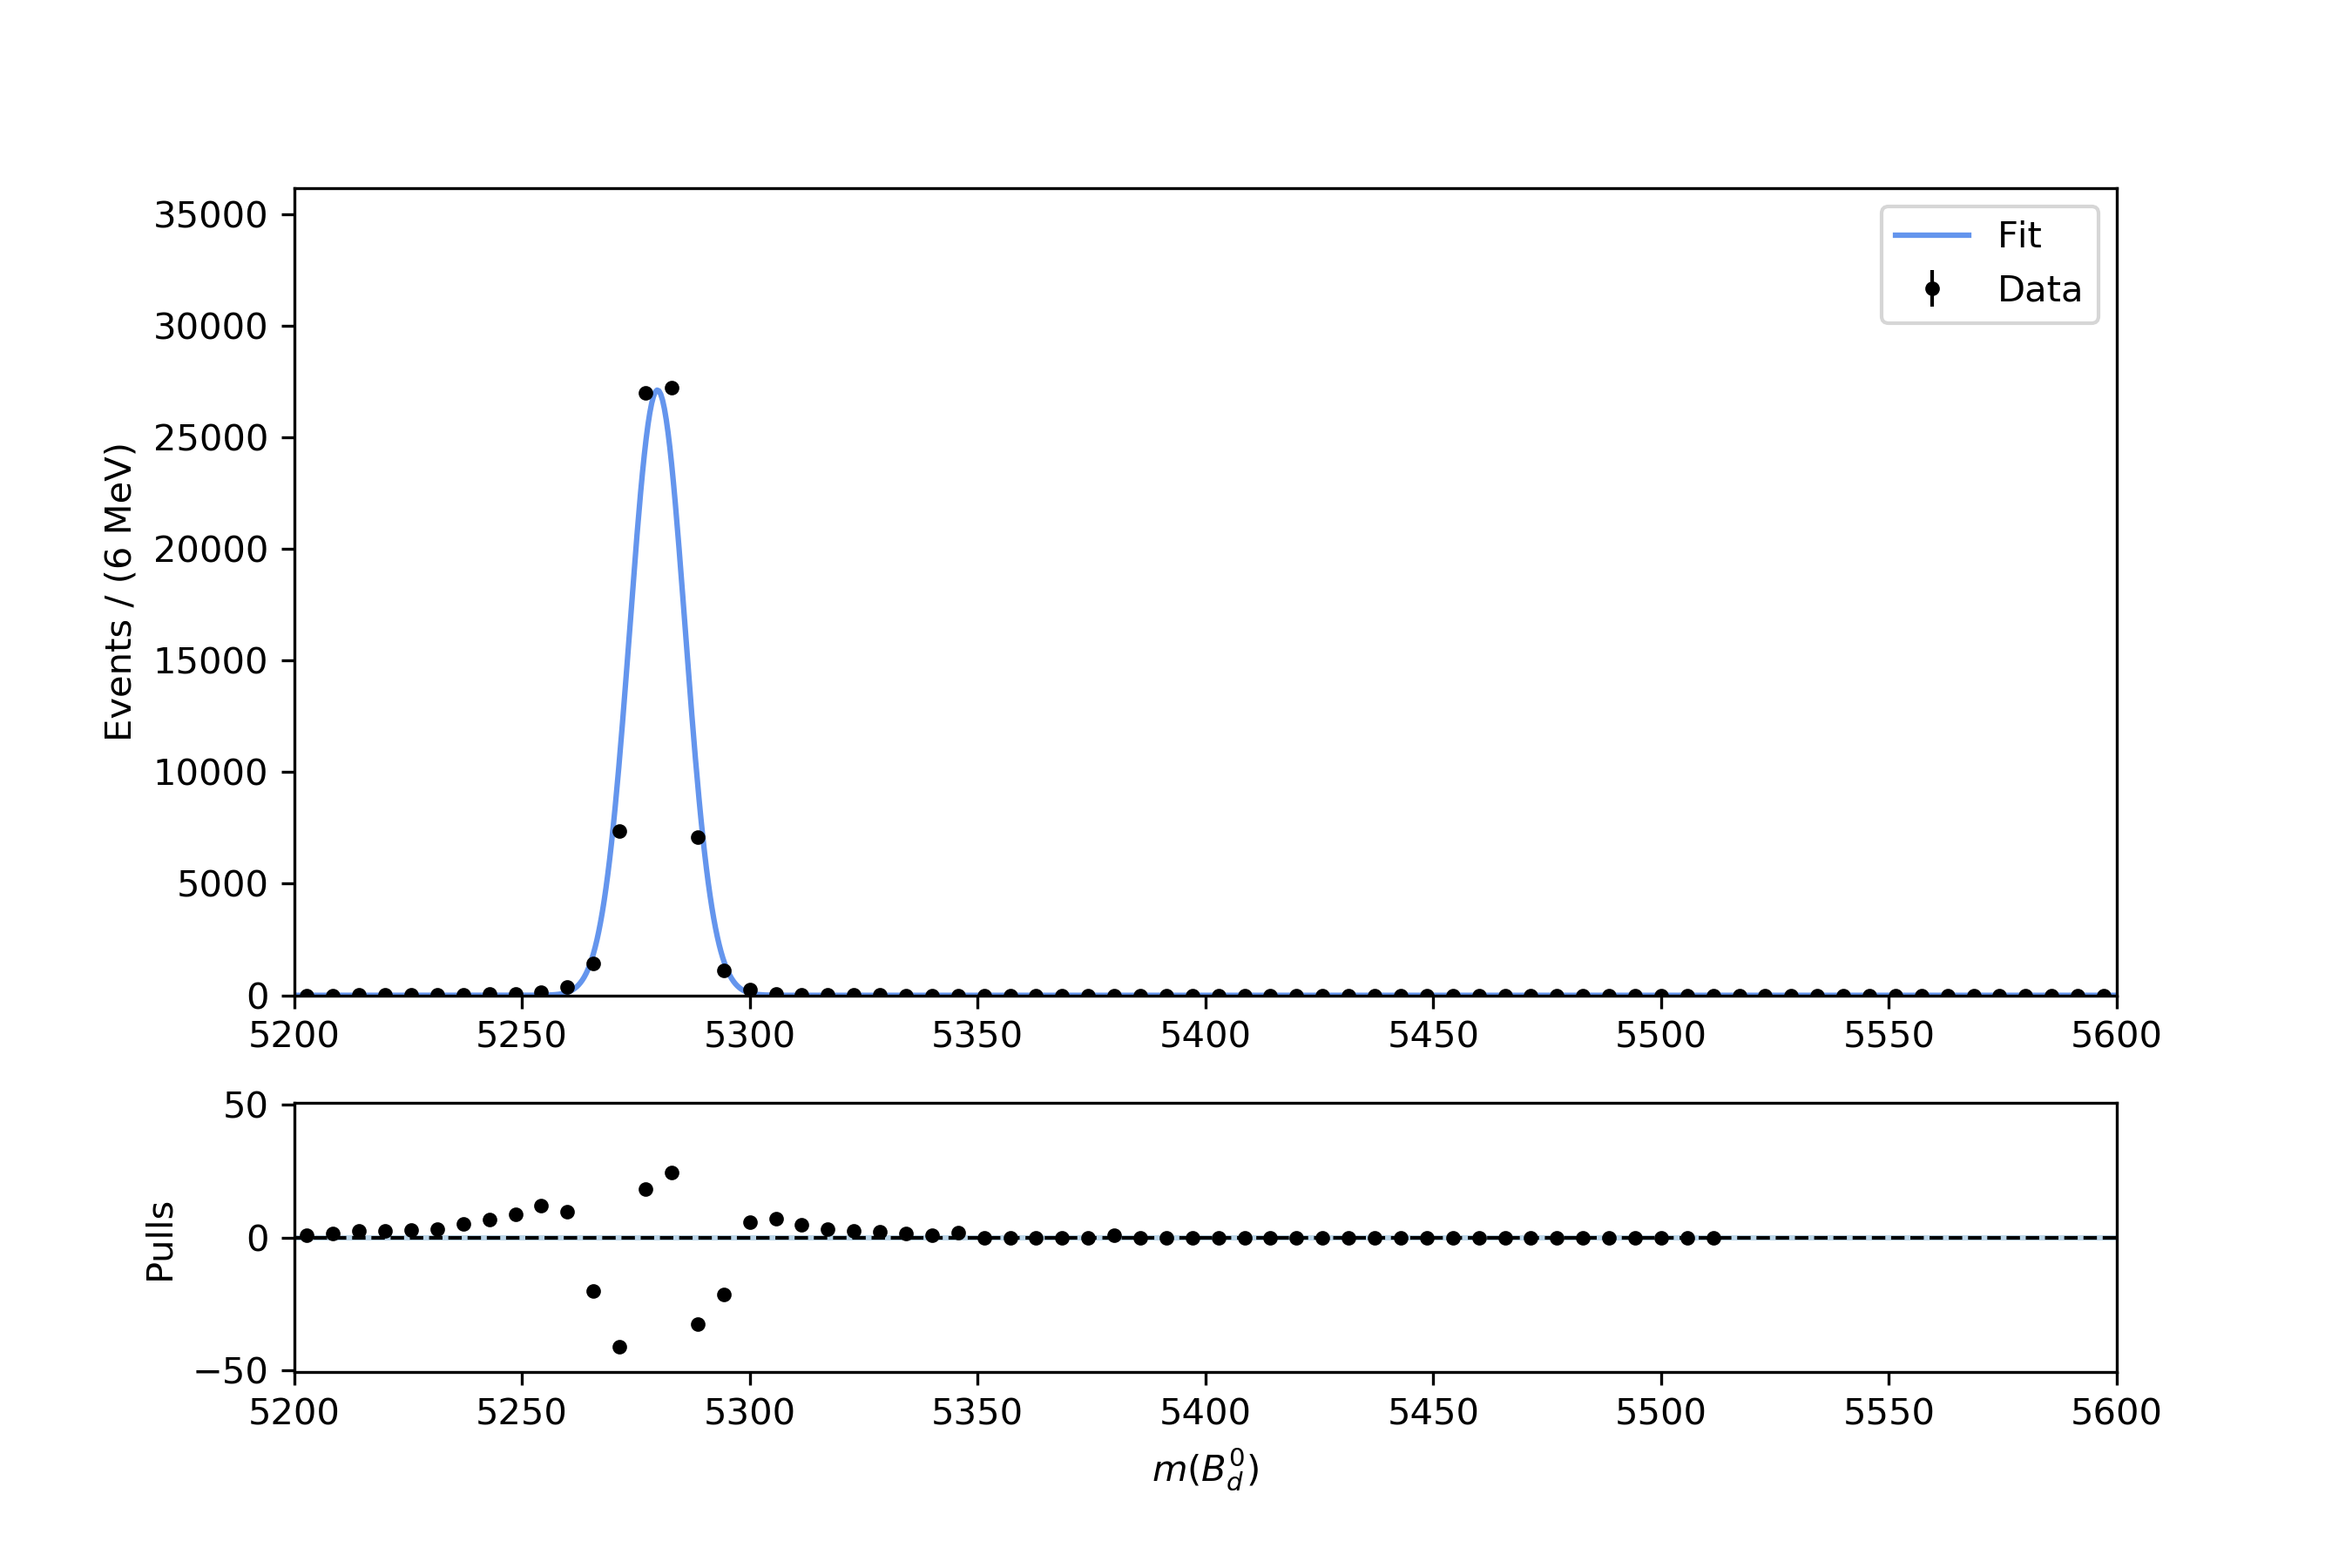
\includegraphics[width=0.99\linewidth]{Figure/third.png}
            \caption{Control simulation.}
            \label{fit_control_peak}
        \end{subfigure}
        \caption{Fitted peak to the signal and control simulation.}
    \end{figure}

    When considering the full mass window of the real data sample, the shapes obtained from the preliminary fits on simulations along with an exponential background are shown in Figure \ref{sec_last}. An exponential background refers to a type of background distribution in data that decays exponentially. This can be represented mathematically as:\\

    \begin{align}
        f(x)=Ae^{-\lambda x}
    \end{align}

    where A is the normalization constant, $\lambda$ is the decay constant and x is the observable.\\
    
    \begin{figure}[H]
        \centering
        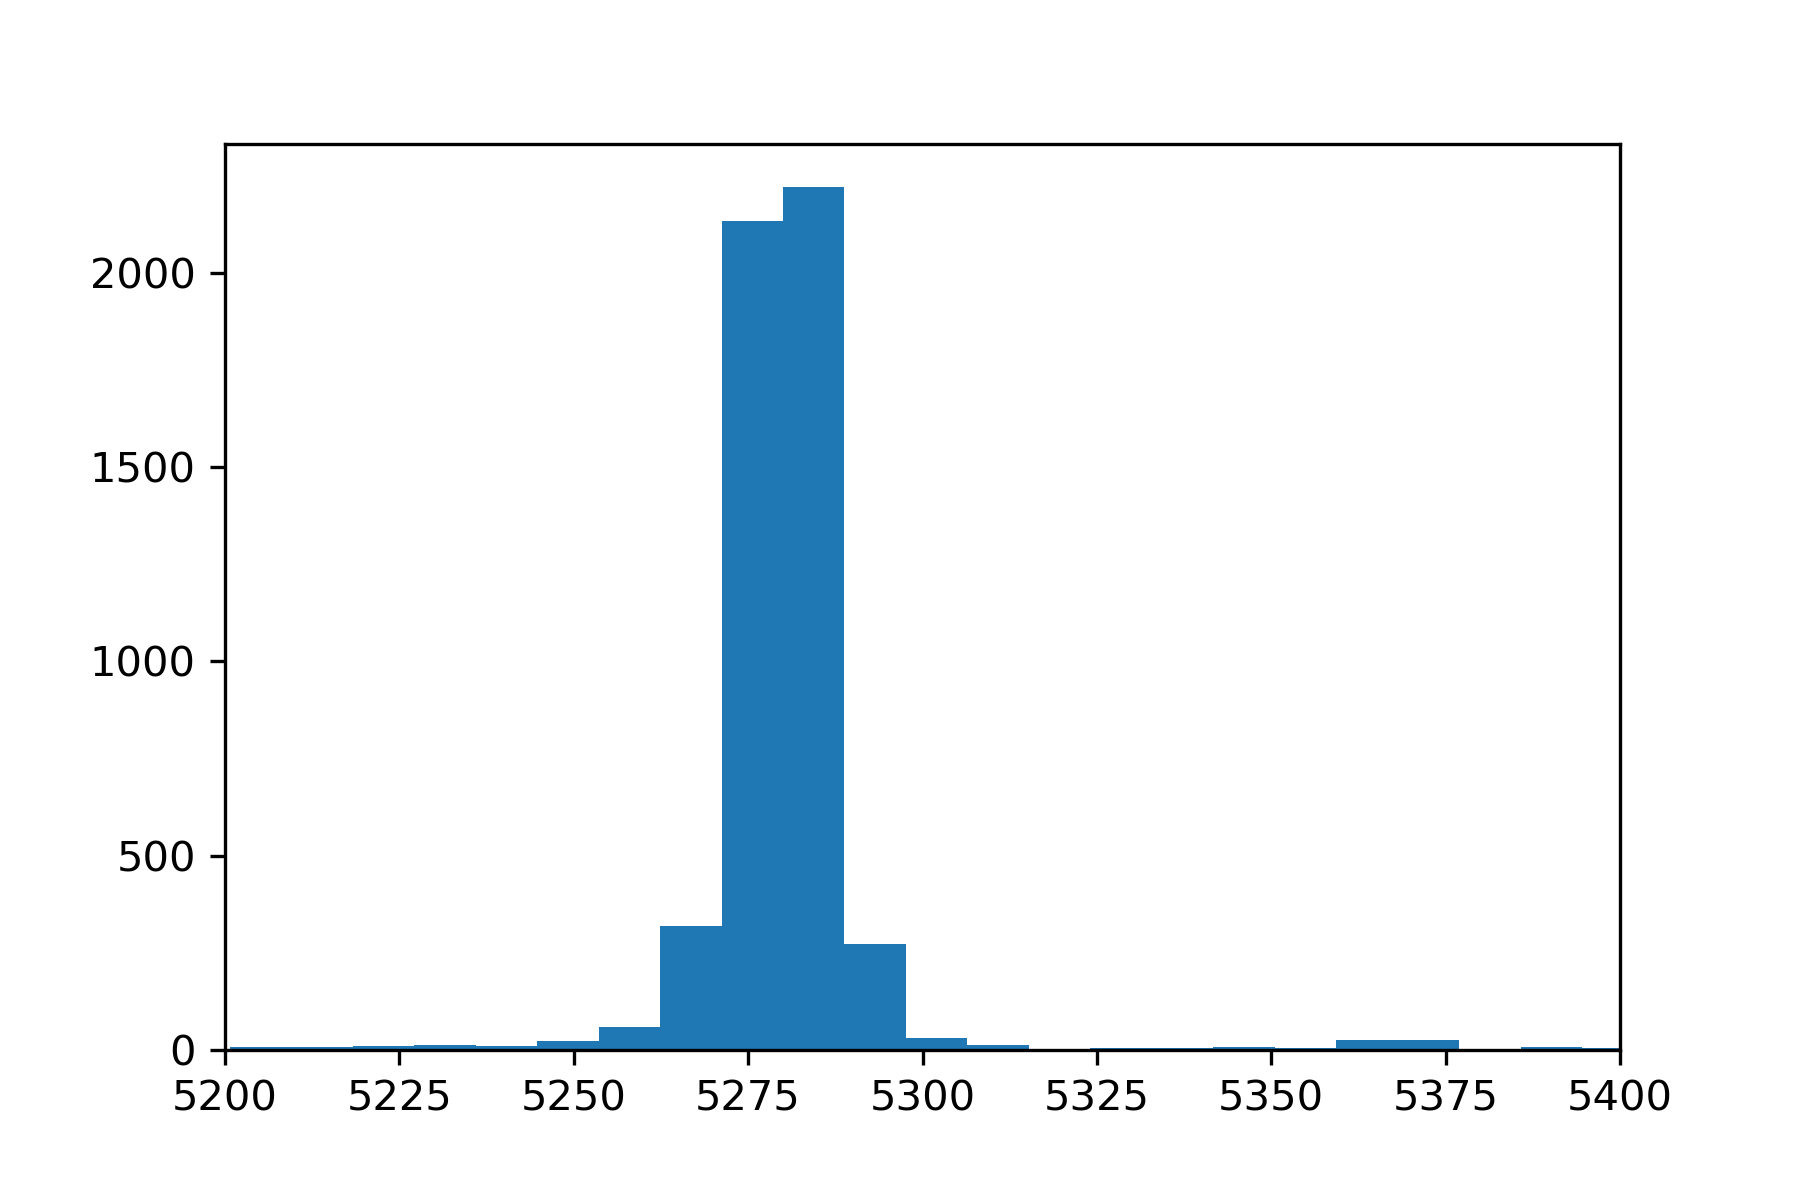
\includegraphics[width=0.8\linewidth]{Figure/second_last.png}
        \caption{Full data fitted with fixed peak shapes and exponential background.}
        \label{sec_last}
    \end{figure}
    Figure \ref{final} shows the invariant mass distribution of candidates from the real data sample which were selected via the classifier criteria. The results of the fit are overlaid.\\
    \begin{figure}[H]
        \centering
        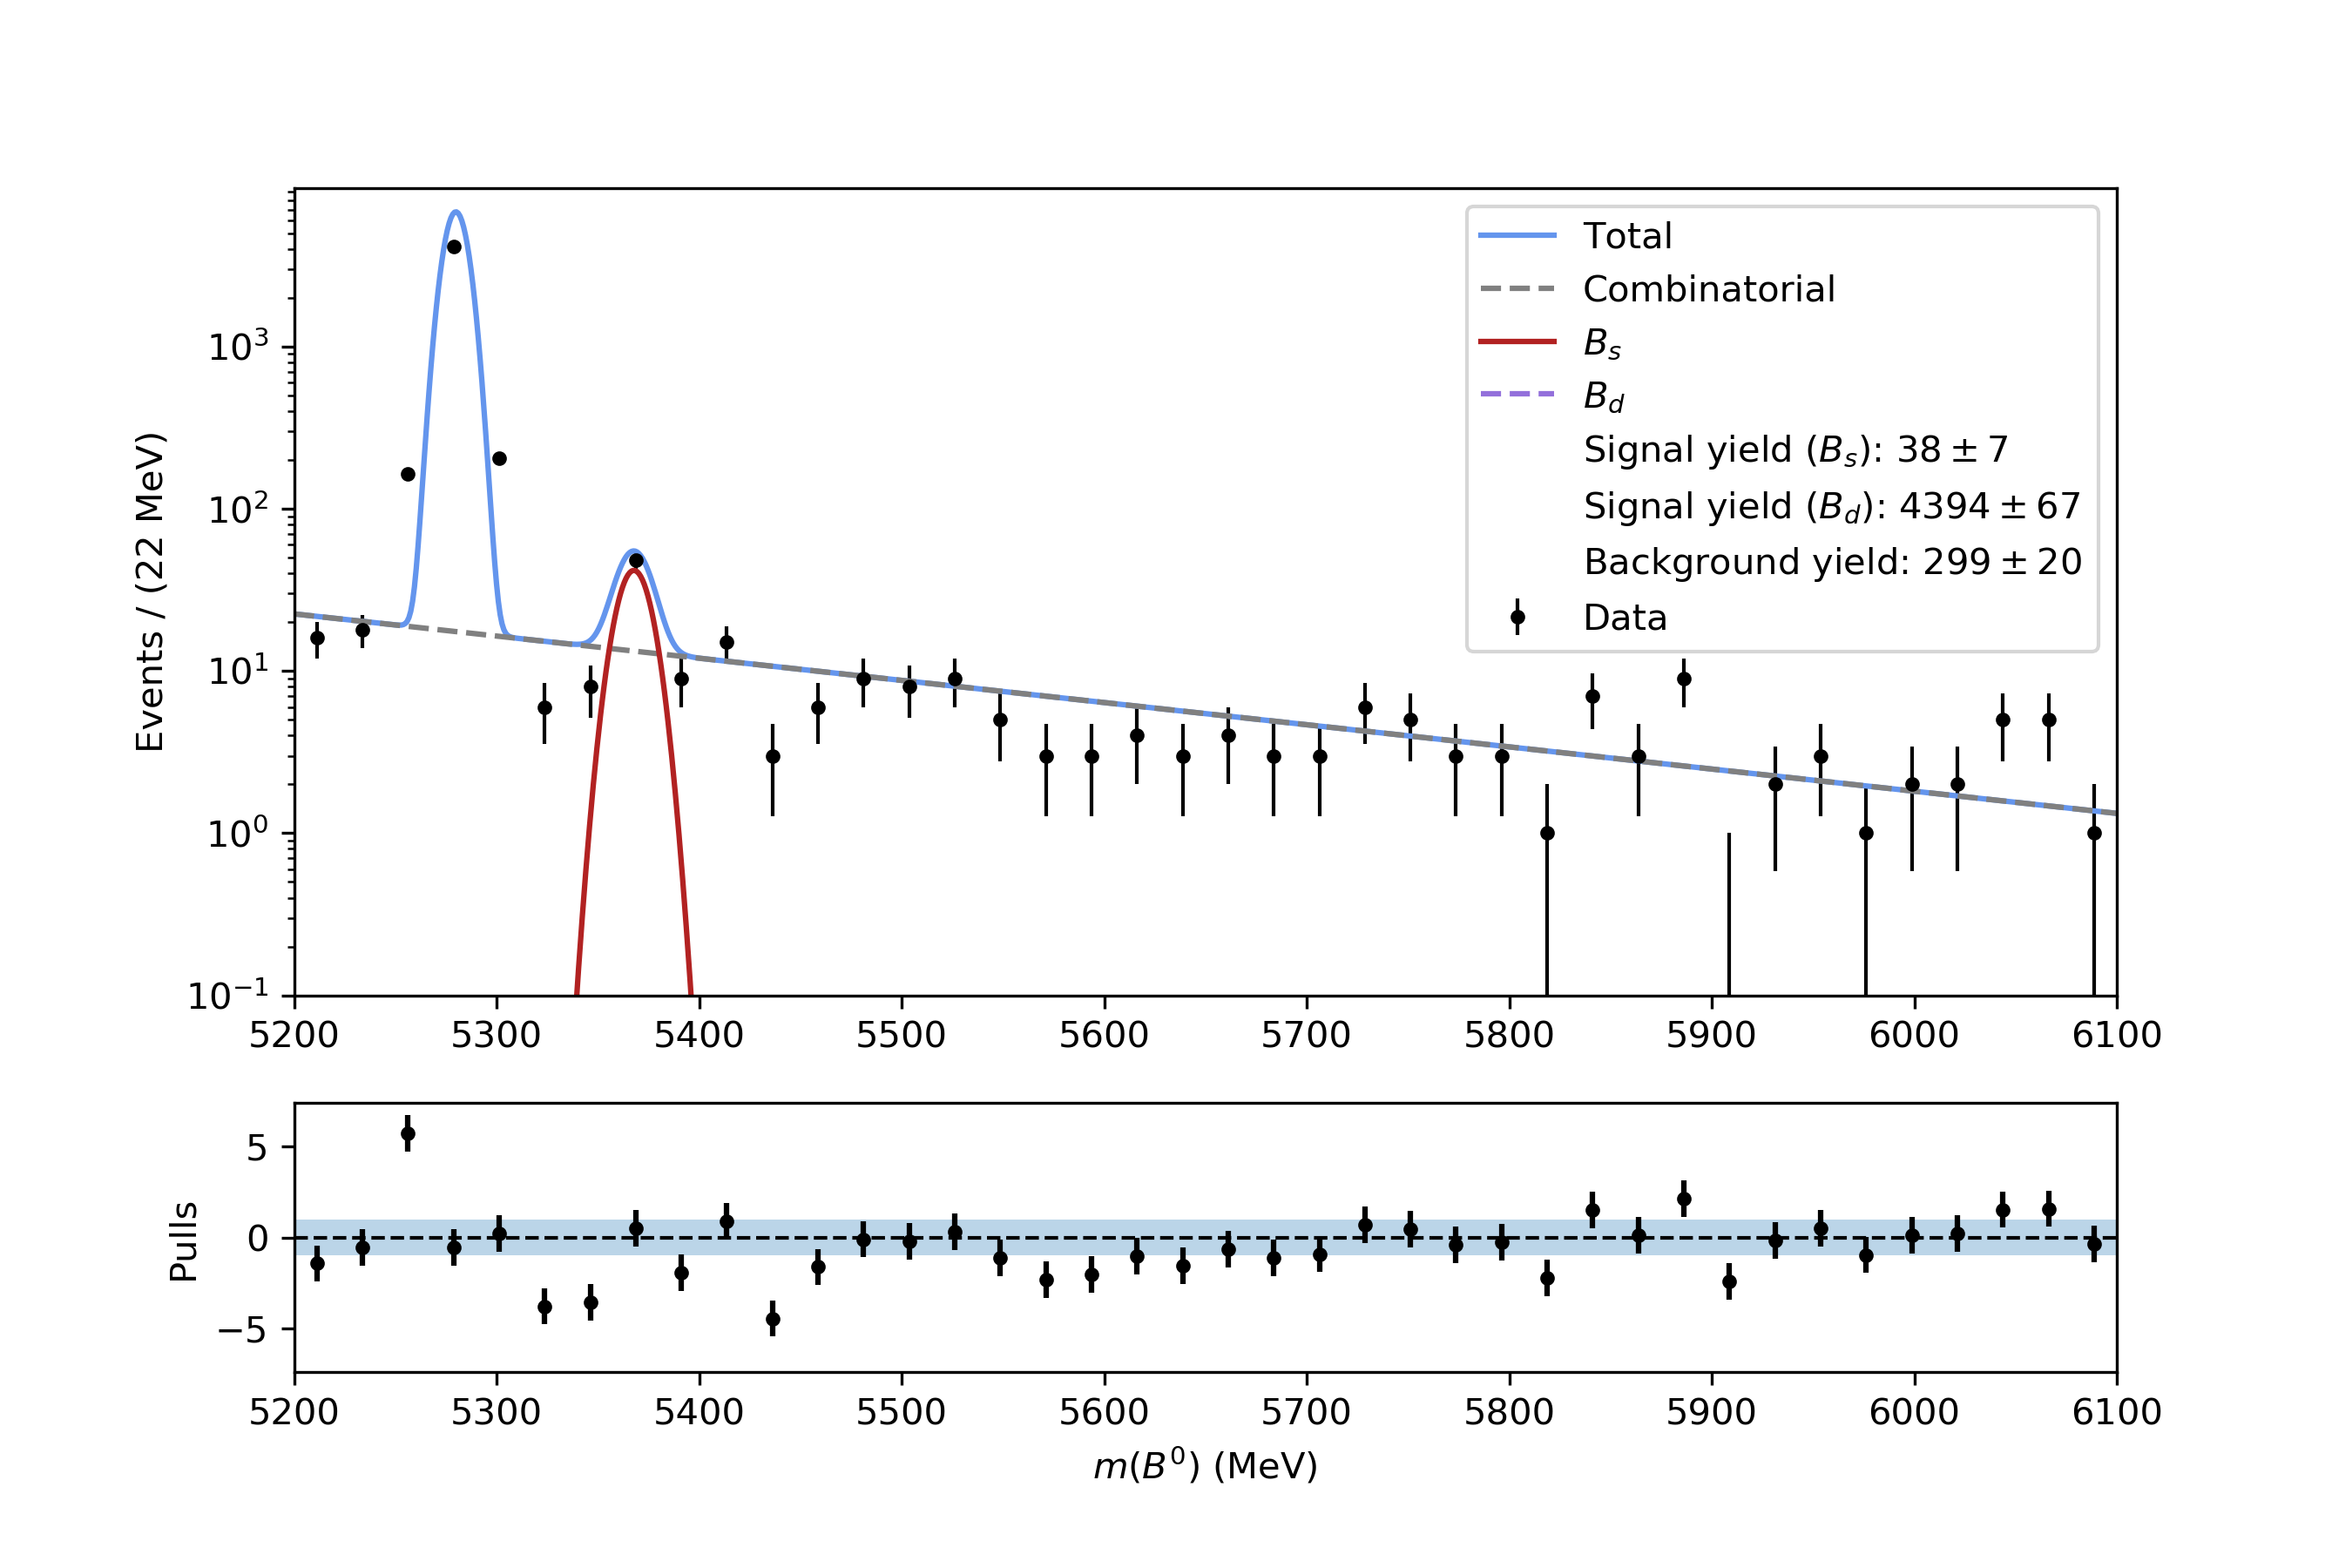
\includegraphics[width=0.8\linewidth]{Figure/final_fit.png}
        \caption{Full mass window of the real dataset using the shapes obtained from the preliminary fits on the simulations and an exponential background.}
        \label{final}
    \end{figure}
    Using the values, obtained from the fit, the proxy significance can be calculated. The signal and background events in the signal region are $n_{sig}=30$ and $n_{bkg}=17$ respectively. Hence, according to Eqn.\ref{proxy}, the signal significance is 4.42.\\
    